\documentclass{include/tfgitic}[2022/06/30]

% Per a mostrar dues imatges en una sola figura.
\usepackage{subcaption}
% Per a mostrar el símbol de Euro
\usepackage{eurosym}
\DeclareSIUnit{\EUR}{\text{\euro}}
% Per a arbres de dependències
\usepackage[edges]{forest}
% Per a que l'arbre de dependències no surti dels marges
\usepackage{adjustbox}

\addbibresource{misc/tfg.bib}

\title{Implementació d'una pantalla inte\l.ligent}
\subtitle{Creació d'un dispositiu i programari que actualitzi l'orientació
          d'una pantalla al rotar-la}

\author{Eric Roy Almonacid}
\advisor{Francisco del Águila López}

\dedication{Per l'avi, que hagués sigut el primer comprador d'aquest producte}

\begin{acknowledgments}
    Aquest treball no hagués existit si no fos per l'Isaac Iglesias, que em va
    proposar fer aquest projecte, i a poc a poc ha vist com la seva idea anava
    convertint-se en un producte.

    Una altra persona a qui dec aquest treball és al meu tutor del projecte, el
    Francisco del Águila, que m'ha orientat i recolzat durant tot aquest procés.

    També voldria agrair al professorat de l'\acro{epsem}, però en especial al
    Joan Martínez que, juntamtent amb el meu tutor, m'ha aconsellat durant el
    disseny de la placa de circuit imprès.

    L'absència de faltes lingüístiques en aquest document és un mèrit de la
    meva parella, l'Aida Vers, que ha realitzat una correcció exhaustiva del
    treabll.

    Finalment, vull donar les gràcies a totes les persones del meu entorn
    quotidià que, potser fins i tot sense ells saber-ho, han fet que aquests
    mesos no semblin tan durs. Familiars, amics, companys de feina i d'estudis,
    aquest treball també és vostre.
\end{acknowledgments}

\begin{resum}
    La tendència a generar contingut audiovisual en format vertical és una de
    les diverses causes per la qual la gent es plantegi tenir una pantalla de
    l'ordinador en aquesta nova orientació. 
    Una de les solucions més senzilles i econòmiques és adquirir un suport de
    monitor que permeti rotar la pantalla sense haver-la de desmuntar, i així
    disposar fàcilment de les dues orientacions.

    Un inconvenient d'aquest sistema és que, quan es gira la pantalla, s'ha de
    reconfigurar l'entorn gràfic per adaptar-lo a la nova orientació.
    Existeixen alguns monitors d'alta gamma que, mitjançant la connexió d'imatge
    ja existent, poden notificar l'ordinador els canvis d'orientació. Tanmateix,
    aquests sistemes només funcionen correctament si s'utilitza el suport de
    pantalla i protocols recomanats.

    Aquest projecte proposa un dispositiu de baix cost que, mitjançant un sensor
    giroscòpic i una connexió \acro{usb}, detecta l'orientació de la pantalla i
    configura l'entorn gràfic adequadament. S'ha posat èmfasi en l'ús de
    protocols estàndards existents, la compatibilitat entre diferents sistemes
    operatius i la facilitat d'insta\l.lació i ús dels programes relacionats
    amb el dispositiu.
\end{resum}

\begin{abstract}
    The trend towards generating audiovisual content in vertical format is one
    of the various reasons why people consider having a computer screen in this
    new orientation.
    One of the simplest and most economical solutions is to acquire a monitor
    stand that allows the screen to be rotated without having to disassemble it,
    thus easily providing both orientations.

    One drawback of this system is that when the screen is rotated, the graphic
    environment needs to be reconfigured to adapt to the new orientation.
    There are some high-end monitors that, through the existing image
    connection, can notify the computer of orientation changes. However,
    these systems only work properly if the recommended screen support and
    protocols are used.

    This project proposes a low-cost device that, using a gyroscope sensor and a
    \acro{usb} connection, detects the screen orientation and configures the graphic
    environment accordingly. Emphasis has been placed on the use of existing
    standard protocols, compatibility between different operating systems, and
    the ease of installation and use of device-related programs.
\end{abstract}

\begin{document}

%\part{Memòria}

\chapter{Introducció}
\label{cap:introduccio}

Durant els darrers anys, el contingut digital en format vertical no ha cessat
d'augmentar, sent una de les principals causes l'ús generalitzat dels
dispositius mòbils \cite{Navarro2023El}. Les xarxes socials no van tardar a
adaptar les seves interfícies a aquestes noves resolucions. De fet, aquesta
tendència també s'ha portat a moltes altres aplicacions, tan de mòbil com
d'escriptori. Per exemple, han nascut termes com el
\est{Mobile-First Web Design}, que incita als desenvolupadors de pàgines web
a dissenyar les pàgines per a dispositius mòbils, i adaptar-les després
(el contrari del que es feia tradicionalment) \cite{varrela2015mobile}.

Tot plegat ha creat una nova moda: tenir una pantalla en vertical
en un ordinador de sobretaula. La majoria de monitors es poden muntar en
aquesta orientació sense necessitar un altre suport, pel que aquesta pràctica
s'ha popularitzat molt fàcilment \cite{WeardenPortrait}.
Disposar d'una pentalla en vertical també pot aportar altres avantatges. Per
exemple: els desenvolupadors poden veure més línies d'un mateix fitxer de codi
a la vegada, els dissenyadors de cartells o continguts per a dispositius mòbils
també poden beneficiar-se d'aquesta orientació.

Tanmateix, de vegades pot resultar més útil veure contingut en format
horizontal, com per exemple les pe\l.lícules. Si disposem de la configuració
anterior, hauríem de desmuntar la pantalla del suport i tornar-la a co\l.locar
en l'orientació desitjada. Un cop fet això, s'hauria d'anar a la configuració
del sistema per a que l'entorn gràfic del sistema operatiu mostri els continguts
d'aquella pantalla correctament. Aquest cúmul de tasques fan aquest procediment
tediós, sent aquest un motiu pel que no es sol dur a terme.

Per a resoldre aquest problema, han sortit a la venda suports rotatoris per a 
monitors \cite{DIGITUSUniversal}. Aquests redueixen el problema mencionat
anteriorment a només haver de girar la pantalla amb la força de la mà, i
configurar l'entorn gràfic. Algunes marques han anat més enllà, oferint
monitors incorporats amb un sensor de gravetat que, al detectar un canvi
d'orientació s'encarreguen d'actualitzar l'entorn gràfic \cite{LCLC}.

Malauradament, aquests últims tipus de productes tenen alguns punts negatius:
\begin{itemize}
    \item El fabricant només assegura que s'actualitzi l'orientació en l'entorn
    gràfic si el sistema operatiu és Windows.
    \item Aquest sistema d'actualització funciona per sobre del protocol de
    transmissió de l'imatge (en aquest cas, \acro{hdmi}), i no es garanteix el correcte
    funcionament en altres connexions.
    \item Finalment, s'ha de comprar una nova pantalla per a poder gaudir del
    sistema. És a dir, el fabricant no ven per separat un dispositiu que tingués
    el mateix propòsit i pugués allargar la vida útil d'una pantalla ja
    comprada.
\end{itemize}

Així doncs, l'objectiu principal d'aquest treball és crear un dispositiu que,
juntament amb un suport rotatori ja existent, pugui convertir la tasca de girar
el monitor en un gest habitual durant una rutina de treball. Es posarà èmfasi en
la facilitat d'insta\l.lació i ús, compatibilitat amb diferents sistemes
operatius, i a una hipotètica comercialització del producte.

Com és d'esperar, al mercat també hi ha sensors d'orientació i/o acceleròmetres
\acro{usb} \cite{Yocto3D}. Tanmateix, gairebé la totalitat d'ells utilitzen
\est{drivers} propis i no es basen en estàndards preestablerts, que acostumen
a reduir el temps de desenvolupament i millorar la robustesa del sistema. S'ha
decidit doncs que s'utilitzarà aquests dispositius com a referència per a
comparar els resultats que s'obtindran, però es crearà un dispositiu des de zero.

La motivació darrera l'elecció d'aquest treball rau en l'interès personal en
posar en pràctica totes les àrees de coneixement que composen la titulació que
s'està cursant. Adicionalment, també hi havia un interès personal per a obtenir
un producte final que pot aportar un ús en el dia a dia. Per aquest motiu, quan
es va presentar l'oportunitat de dissenyar el producte mencionat anteriorment,
es va pensar que era una molt bona manera per a donar un final rodó al grau.

Aquesta documentació s'haurà de complementar amb el codi font del projecte, que
segurament es trobarà juntament amb aquest fitxer. En cas que no es disposi o
es vulgui consultar la darrera versió, es trobarà el codi font a
\url{https://github.com/royalmo/gyroscreen}.
Finalment, es vol mencionar que aquest document s'ha generat amb l'eina \LaTeX,
i es poden consultar els fitxers font a \url{https://github.com/royalmo/tfg}.

\chapter{Objectius}
\label{cap:objectius}

\section{Objectius generals}

L'objectiu principal d'aquest treball de fi de grau és implementar un dispositiu
de dimensions reduïdes, que s'enganxarà darrere el monitor i es connectarà
a l'ordinador mitjançant un cable \acro{usb}. Aquest dispositiu contindrà els
sensors i altres components necessaris per poder informar l'ordinador sobre
l'orientació actual de la pantalla. A través d'un programari propi i de la
interfície de programació que proporciona l'entorn gràfic, es canviarà
l'orientació de la pantalla en funció de les dades rebudes del dispositiu. Es
buscarà sempre la màxima compatibilitat possible, facilitat d'insta\l.lació i
ús quotidià, i un preu de construcció raonable.


\section{Objectius específics}

Aquest treball de fi de grau es podria estendre molt més enllà dels pocs mesos
de temps dels que es disposa. Per això, es definiran uns objectius essencials
per considerar el projecte completat, i uns objectius addicionals o
ampliacions que, tot i no ser troncals pel projecte, poden completar o
millorar el sistema.

Objectius essencials:
\begin{itemize}
    \item Fer una recerca sobre la tecnologia i pràctiques actuals sobre el 
    procés de disseny de dispositius \acro{usb}.
    \item Escollir els components electrònics del dispositiu i dissenyar una
    placa de circuit imprès. S'imprimiran unes quantes plaques per poder fer
    proves del sistema complet.
    \item Definir la forma en què l'usuari podrà insta\l.lar i configurar
    el sistema.
    \item Adaptar una implementació o implementar el programari que comunicarà
    el dispositiu i l'ordinador. Aquesta aplicació haurà de complir els
    requisits d'interacció de l'usuari definits en el punt anterior. En aquest
    punt es centrarà només en l'entorn de GNU/Linux.
\end{itemize}

Objectius addicionals:
\begin{itemize}
    \item Adaptar el sistema a Windows i MacOS fent-lo, doncs, compatible amb la
    gran majoria de sistemes operatius del mercat.
    \item Un cop es tingui la placa, dissenyar i construir una carcassa pel
    dispositiu.
    \item Dissenyar i implementar una interfície d'usuari senzilla i amable
    que permeti configurar el dispositiu.
    \item Realitzar un estudi econòmic per a una possible comercialització del
    projecte.
    \item Dissenyar una pàgina web senzilla per promocionar el projecte.
    \item Preparar el sistema per poder acceptar més d'un dispositiu
    simultàniament.
\end{itemize}

\chapter{Estat de l'art}
\label{cap:estat-de-l-art}

Aquest capítol té per objectiu resumir i ordenar de forma estructurada la
recerca inicial que s'ha fet per a aquest projecte. Només es posarà èmfasi en
les parts rellevants per al projecte, però sempre s'inclourà alguna referència
per complementar o ampliar algun concepte.

\section{Protocol USB}

Sent la connexió \acro{usb} un dels punts més cèntrics d'aquest treball de
fi de grau, s'ha iniciat la recerca per aquest cantó. No només s'ha escollit
usar aquest estàndard per la seva compatibilitat
i les facilitats que proporciona a l'usuari, sinó que també hi havia un interès
personal en entendre aquest protocol.

L'\acro{usb}, que significa \est{Universal Serial Bus} en anglès, és un
estàndard de comunicació que permet la connexió, intercanvi i transferència de
dades entre dispositius electrònics com ara ordinadors, telèfons mòbils, i
impressores. Aquesta tecnologia utilitza uns connectors estàndards que són
àmpliament reconeguts per la seva facilitat d'ús i versatilitat en una àmplia
gamma d'aplicacions. Els dispositius \acro{usb} poden transmetre dades a
diferents velocitats, des de velocitats molt baixes fins a velocitats molt
altes, i són compatibles amb una gran varietat de sistemes operatius i
maquinari \cite{Axelson2015USB}.

\subsection{Arquitectura}

L'arquitectura del \acro{usb} és de tipus mestre-esclau, en què el mestre sol ser
l'ordinador i l'esclau el dispositiu que es connecta. Com es veurà a l'Apartat
\ref{sec:usb_versions}, s'acabarà utilitzant la versió \acro{usb2}. Per
evitar fer molt extens aquest document, només es detallarà l'arquitectura
d'aquesta versió.

\subsubsection*{Aspectes físics}
\label{subsub:usb_physic}

El baix nivell no es detallarà en excés, ja que s'utilitzaran llibreries que
compleixen l'estàndard des d'un nivell més alt. Tanmateix, s'ha trobat
interessant fer una pinzellada de l'estàndard.

El connector \acro{usb2} està compost de quatre cables: \acro{5v}, \acro{gnd},
\acro{d+} i \acro{d-}. La funció del cable de \acro{5v} és alimentar el
dispositiu, amb una intensitat de fins a
\SI[round-mode=places,round-precision=0]{500}{\milli\ampere}. Aquestes
prestacions de corrent resulten ser suficients per a la major part dels
dispositius que compleixen l'estàndard. Sabent que \acro{gnd} és el cable
necessari per tancar els circuits, només queda \acro{d+} i \acro{d-} per
enviar dades.

Contràriament al que es podria pensar, el flux de dades (i electricitat) no
està predefinit: en un moment pot ser l'ordinador el que utilitzi els dos cables
per transmetre dades al dispositiu, i en un altre pot ser a l'inrevés. De fet,
els dos cables sempre envien el mateix, però de manera invertida; això es coneix
com a tensió en mode diferencial. D'aquesta manera, les interferències en mode
comú (respecte
\acro{gnd}) es poden eliminar (restant els dos senyals). La tensió en mode
diferencial funciona de forma òptima si els dos cables estan trenats (d'aquesta
forma reben gairebé la mateixa interferència, que s'anu\l.la quan es fa la
resta) \cite{DiffTension}.

És important tenir en compte que la tensió d'operació de l'estàndard \acro{usb2}
és de
\SI[round-mode=places,round-precision=1]{3.3}{\volt}, encara que la tensió que
proporciona el cable d'alimentació sigui de
\SI[round-mode=places,round-precision=0]{5}{\volt}.
Aquest detall serà molt important de cara
al disseny del dispositiu, ja que implicarà, molt probablement, l'ús de dos
díodes Zener a l'entrada de les línies de transmissió de dades.

A la figura \ref{fig:usb-wave} es pot veure un exemple de transacció \acro{usb}.
Hi ha un preàmbul per sincronitzar el rellotge dels dos dispositius i una
transmissió de dades fins que \acro{d+} i \acro{d-} deixen de tenir valors
invertits.

\begin{figure}[ht]
    \centering
    \includegraphics[width=0.8\textwidth]{images/usb_signal_example.png}
    \caption{Exemple de transmissió \acro{usb}. \cite{Contributors2024USB}}
    \label{fig:usb-wave}
\end{figure}

\subsubsection*{Transaccions}

Tal com s'ha comentat en l'apartat anterior, el canal de transmissió que
proporciona l'estàndard és unidireccional o \est{half-duplex}. En aquest
apartat es defineixen els tres tipus de transaccions.

Una transacció és un seguit d'intercanvi de dades entre l'ordinador i el
dispositiu. Totes s'inicien des de l'ordinador, encara que el paquet que es
vulgui enviar sigui en sentit invers. No s'entra en detall sobre el protocol de
connexió, ja que per aquest treball no té importància.

Existeixen tres tipus de transaccions:
\begin{itemize}
    \item Les transaccions \emph{out} serveixen per enviar paquets de
    l'ordinador al dispositiu.
    \item Les transaccions \emph{in} serveixen per enviar paquets del
    dispositiu a l'ordinador. A diferència del tipus anterior, aquesta
    transacció no la inicia qui vol enviar el paquet. Per poder
    superar aquest obstacle s'utilitza el següent tipus.
    \item Les transaccions de control serveixen per poder esbrinar quan el
    dispositiu necessita enviar dades, pactar velocitats de transmissió, entre
    d'altres. La transacció de control més important és la \emph{setup},
    que serveix per intercanviar informació inicial entre els dispositius. Més
    endavant es veuran els tipus de dades que s'intercanvien inicialment.
\end{itemize}

L'important d'aquest apartat és tenir present que les transaccions \emph{in} i
\emph{out} es van dissenyar per mantenir un intercanvi de dades constant,
mentre que les transaccions de control, fora de l'etapa de \emph{setup}, estan
més pensades per a petits intercanvis de dades, i més irregulars. Més endavant,
aquesta informació resultarà important per entendre la implementació del
dispositiu.

\subsubsection*{Modes de transmissió}

Un mode de transmissió és una descripció de quines transaccions i quan s'han
d'enviar per aconseguir un objectiu específic. Existeixen quatre modes
de transacció, descrits en la taula \ref{tab:transmision-modes}.

\begin{figure}[ht]
    \centering
    \begin{tabular}{l p{0.6\linewidth}}
        \toprule
        \textbf{Mode}           & \textbf{Descripció} \\
        \midrule
        Control & Mode utilitzat durant la configuració del dispositiu per a enviar comandes específiques que requereix el protocol. \\
        Isòcron & Mode utilitzat per a transmetre dades a temps real (audio, vídeo, \dots). Aquest mode reserva una porció de l'ample de banda \acro{usb} per a garantir la mateixa latència. No es tornen a enviar paquets amb errors. \\
        Per interrupció & Aquest mode demana als dispositius cada cert temps si han de transmetre dades. Utilitzat per a dispositius que requereixen transmetre poques dades, com teclats o ratolins. \\
        Massiu (\est{Bulk}) & Mode utilitzat per a dispositius que necessiten transmetre moltes dades i garantir l'absència d'errors, però que no tenen requeriments de latència. Ho són, per exemple, les impressores i els discs durs. \\
        \bottomrule
    \end{tabular}
    \caption{Modes de transmissió \acro{usb} \cite{Axelson2015USB}.}
    \label{tab:transmision-modes}
\end{figure}


Com es pot veure, amb aquests modes ja es cobreixen gairebé la totalitat dels
usos típics del protocol \acro{usb}: un micròfon o altaveu, un sensor, un
disc dur, entre d'altres. En el cas del dispositiu que es vol crear, el mode més
adequat és el d'interrupcions, ja que el sensor farà lectures a una freqüència
constant.

\subsubsection*{Metadades}
\label{subsubsec:metadades}

Durant els intercanvis inicials, durant l'etapa \emph{setup}, el dispositiu
comparteix certes metadades a l'ordinador, fet que li permet identificar-se
i descriure les especificacions necessàries. Un dels avantatges més visibles
d'aquest procés invisible és la funcionalitat \est{plug\&play}, que evita
insta\l.lar programari per a cada nou dispositiu que es connecta. El paquet
que s'intercanvia inicialment s'anomena \emph{Descriptor de dispositiu}.

Dos codis molt importants en aquest procés són el \acro{vid} i el \acro{pid},
acrònims de \est{Vendor ID} i \est{Product ID}. El \acro{vid} identifica
l'organisme que ha emès el dispositiu, i el \acro{pid} identifica el producte.
Cal tenir present que aquests dos codis són idèntics per a tots els dispositius
que es produeixin, per la qual cosa no té res a veure amb un número de sèrie. El motiu
pel qual es divideix el codi en dos nombres diferents recau en la forma en què
s'assignen als dispositius, tal com s'explicarà més endavant. Tanmateix,
a efectes tècnics es considera com un únic nombre.

Aquests codis tenen per objectiu que l'ordinador pugui identificar el tipus de
dispositiu que s'ha connectat. Un dels usos principals d'aquesta funcionalitat
és la creació de regles \acro{udev}, que en els sistemes de Linux assignen
\est{drivers} en funció dels codis anteriorment esmentats.

Una altra metadada que s'intercanvia a l'inici de la connexió és la classe
de dispositiu. Aquesta pot diferenciar entre dispositius multimedia, Hubs
\acro{usb}, teclats i ratolins, etcètera. Un dels grups més grans és el
\acro{hid}, o \est{Human Interface Devices}, una classe de dispositiu tan
versàtil que també s'utilitza en el protocol \est{Bluetooth}. S'explicarà amb
detall la classe \acro{hid} a l'apartat \ref{sec:hut}.

Finalment, hi ha altres metadades que poden ser interessants de conèixer, com
poden ser les freqüències en què el dispositiu envia dades o versions de
l'estàndard.

\subsubsection*{Interfícies i \est{Endpoints}}

Dintre de les metadades que s'envien en el descriptor de dispositiu hi ha els
descriptors de configuració. Aquests poden tenir una o diverses interfícies, que
al seu torn poden tenir un o més \est{endpoints}. Tot plegat queda amb una
jerarquia, tal com es pot veure a la figura \ref{fig:usb-endpoints}.

\begin{figure}[ht]
    \centering
    \begin{adjustbox}{width=\linewidth}
    \begin{forest}
        forked edges,
        for tree={draw,align=center,edge={-latex}}
        [Device Descriptor
            [Configuration Descriptor 1
                [Interface 0
                    [Endpoint 1]
                    [Endpoint 2]
                    [\dots]
                ]
                [Interface 1
                    [Endpoint 1]
                    [\dots]
                ]
                [\dots]
            ]
            [Configuration Descriptor 2
                [Interface 0]
                [\dots]
            ]
            [\dots]
        ]
    \end{forest}
    \end{adjustbox}

    \caption{Diagrama de jerarquia del descriptor de dispositiu \acro{usb} \cite{Axelson2015USB}.}
    \label{fig:usb-endpoints}
\end{figure}


Es començarà a explicar aquesta estructura des del nivell més baix. Un
\est{endpoint} és un canal de comunicació entre el dispositiu i l'ordinador.
Aquest es configura amb un dels modes mencionats anteriorment. Normalment, es
comença a contar a partir del número 1, donat que es reserva l'\est{endpoint}
0 per a trames de control de la interfície.

És molt comú que un \est{driver} necessiti més d'un \est{endpoint} per
comunicar-se amb el dispositiu. Per exemple, un teclat pot enviar dades de les
tecles premudes a través de l'\est{endpoint} 1 i rebre informació de l'ordinador
(com, per exemple, una ordre per encendre el llum del Bloq Mayus) a través de
l'\est{endpoint} 2. En aquest cas hi ha un \est{endpoint} en mode d'interrupció
i un altre en mode de control (només rebrà trames \est{out} de tant en tant).

Els \est{endpoints} s'agrupen en interfícies. L'ordinador pot tractar cada
interfície independentment i assignar diferents \est{drivers} per a cada una
d'elles. Així doncs, un teclat pot utilitzar el \est{driver} per defecte del
sistema operatiu i a la vegada tenir una interfície amb \est{drivers} específics
per a aquell model concret per tal de, per exemple, fer animacions amb la
retroi\l.luminació. És important utilitzar sempre que es pugui \est{drivers}
estàndards ja que, en el cas concret del teclat, permet que aquest segueixi
funcionant en un sistema operatiu que no disposi dels \est{drivers}
específics (com podria ser un entorn de \acro{bios}).

Finalment, les interfícies es poden agrupar en descriptors de configuració.
Aquests descriptors estan pensats per a dispositius que tenen dos modes
diferenciats, com per exemple un convertidor d'\acro{usb} a Jack d'àudio. Aquest
dispositiu pot funcionar tant d'entrada (connectant un micròfon) com de sortida
(connectant un altaveu), però no d'entrada i de sortida a la vegada. En aquest
cas hi haurà dos descriptors de configuració, i el dispositiu o el sistema
operatiu decidiran quin utilitzar en cada cas.

\subsection{\est{USB Implementers Forum}}
\label{subsec:usb-if}

El logo d'\acro{usb} i les imatges derivades estan sota drets d'autor. L'entitat
que gestiona qui pot utilitzar-los en el seu producte és l'\acro{usb-if},
provinent de l'anglès \est{\acro{Usb} Implementers Forum}. Aquesta entitat està
formada per moltes empreses tecnològiques multinacionals \cite{USBGetting}.
Per poder dir que un producte ofereix connectivitat \acro{usb}, l'empresa
fabricant necessita el permís d'\acro{usb-if}. No només això: per complir
l'estàndard, cal utilitzar un codi \acro{vid} i \acro{pid} únics per a cada
producte (no per a cada dispositiu). Aquests codis també els gestiona aquesta
entitat.

Per poder obtenir els drets d'ús de la imatge d'\acro{usb} i un codi
\acro{VID} (i, en conseqüència, \num[round-mode=places,round-precision=0]{65536}
codis \acro{pid}), s'ha de ser o bé
membre de l'\acro{usb-if} o bé pagar una llicència anual. El
primer dels casos val \SI[round-mode=places,round-precision=0]{5000}{\$}
anualment, mentre que el segon
val \SI[round-mode=places,round-precision=0]{6000}{\$}
%d'entrada i \SI{3500}{\$} cada dos anys
\cite{USBGetting}. Els membres d'\acro{usb-if} també poden participar en les
decisions dels nous estàndards d'\acro{usb}.

Com és d'imaginar, aquestes quotes no són assequibles per a petites empreses
o aficionats que volen treure un producte al mercat. Aquest co\l.lectiu,
generalment, només desitjaria tenir un identificador (\acro{vid} i \acro{pid})
únic per evitar algun possible solapament amb altres productes, però
no sol estar interessat en utilitzar la imatge d'\acro{usb} per promocionar
el seu producte.

Aquest projecte cau en aquest co\l.lectiu. Per decidir com prosseguir, s'ha
observat el que fa la comunitat d'aficionats quan es topa amb aquest problema.
Es recomana llegir la publicació de \cite{Johnson2023usb} si es desitja entendre
els motius d'\acro{usb-if} per posar aquests preus o no cedir \acro{vid}
a projectes de programari i/o maquinari lliure.

Resumidament, en aquests casos es disposa de dues alternatives:

\begin{enumerate}
    \item Inventar-se un \acro{vid} i \acro{pid}: Ja que en cap moment s'ha
    signat cap contracte amb l'\acro{usb-if}, i cap llei vigent ho impedeix, es
    podria escollir un \acro{vid} i \acro{pid} arbitraris i l'\acro{usb-if} no
    podria dir o fer res al respecte. Si s'escull amb cura, la
    probabilitat que els codis escollits co\l.lisionin amb el d'un altre
    producte és molt baixa. Tot i que aquesta metodologia és bona i ràpida per a
    prototips, no es recomana per a productes comercialitzables, en què el risc
    de co\l.lisió és més alt.
    \item Aconseguir un únic \acro{pid}: Les entitats que han comprat un codi
    \acro{vid} a l'\acro{usb-if} disposen de
    \num[round-mode=places,round-precision=0]{65536} codis \acro{pid}. La majoria
    d'entitats no necessiten més d'uns pocs codis \acro{pid}, i poden arribar
    a cedir la resta a projectes com \est{OpenMoko} \cite{OpenMokoUSB}. Aquests
    projectes s'encarreguen d'assignar codis \acro{pid} a altres d'arbitraris.
    Generalment, el seu únic requisit és que el projecte sigui de programari
    i maquinari lliures. Arran d'això, l'\acro{usb-if} va modificar el contracte
    de cessió de codis \acro{vid} l'any 2012, en el qual citava explícitament que no es
    podien cedir codis \acro{pid} a tercers \cite{Johnson2023usb}. Per aquest
    motiu, projectes com \est{OpenMoko} només poden utilitzar com a codis
    \acro{vid} base aquells que s'hagin adquirit abans d'aquest canvi
    de condicions.
\end{enumerate}

El producte d'aquest treball de fi de grau encaixa perfectament en els dos
grups, en funció del moment del projecte: mentre s'estigui desenvolupant, es
pot optar per utilitzar codis definits arbitràriament i, en el moment de
comercialitzar-lo, es pot so\l.licitar un codi \acro{pid} a \est{OpenMoko}.

\subsection{Versions}
\label{sec:usb_versions}

Durant els 30 anys d'\acro{usb-if} han sorgit diferents versions de
l'estàndard. Aquestes es poden dividir en grans grups:

\begin{itemize}
    \item \acro{Usb1}: Aquesta primera versió, projectada l'any 1996, oferia
    una velocitat màxima de transmissió de
    \SI[round-mode=places,round-precision=0]{12}{\mega\bit\per\second}.
    Aquesta versió es considera obsoleta i no s'hi haurien de crear nous dispositius
    amb aquesta.
    \item \acro{Usb2}: La segona versió utilitzava el mateix connector que el
    seu predecessor, però aprofitava els avenços de la tecnologia per
    augmentar la velocitat de transmissió a
    \SI[round-mode=places,round-precision=0]{480}{\mega\bit\per\second}.
    \item \acro{Usb3}: Aquesta versió utilitzava nous connectors, però tots
    eren compatibles amb les versions anteriors. La seva darrera revisió,
    \acro{usb3.2}, pot transmetre dades a
    \SI[round-mode=places,round-precision=0]{20}{\giga\bit\per\second}.
    \item \acro{Usb4}: Encara en fase de desenvolupament, aquesta nova versió
    utilitzaria només el connector \acro{usb-c}, que ja va aparèixer oferint
    compatibilitat fins a l'\acro{usb2}. Es calcula que podria quadruplicar
    la velocitat de transmissió amb relació a l'\acro{usb3.2}.
\end{itemize}

Les versions de l'estàndard estan dissenyades de forma que sempre tenen
compatibilitat envers les anteriors. Per tant, la recomanació general per als
desenvolupadors de dispositius és utilitzar la mínima versió possible, sense
perjudicar el rendiment del dispositiu  \cite{Axelson2015USB}. D'aquesta forma,
el dispositiu podrà funcionar en el nombre màxim d'ordinadors possible.

Sabent que la primera versió està obsoleta, s'ha escollit utilitzar la versió
\acro{usb2} per a aquest projecte, donat que no es necessita transmetre gran
volum de dades.

\subsection{Connectors i cables}

Entre totes les especificacions de l'estàndard \acro{usb} també s'hi troben les
dels cables. Tot i la ignorància general, els allargadors d'\acro{usb}, tinguin
el connector que tinguin, no estan suportats en l'estàndard, i pot ser que
hi hagi interferències \cite{Contributors2024USB}. En canvi, sí que
hi ha definits els \est{Hubs}, que permeten connectar més d'un dispositiu en un
connector, ja que l'electrònica que inclouen eviten pèrdues de dades.

L'estàndard \acro{usb} disposa de diferents connectors. Es poden distingir en
tres grans grups: A, B i C:

\begin{figure}[ht]
    \centering
    \includegraphics[width=0.4\textwidth]{images/usb_connectors.png}
    \caption{Connectors \acro{usb} de tipus A i B. \cite{Contributors2024USB}}
    \label{fig:usb_connectors}
\end{figure}

\begin{itemize}
    \item Els connectors de tipus A són els que es connecten al dispositiu
    que actuarà com a mestre. Existeixen les variants \est{micro} i \est{mini},
    com es pot observar a la Figura \ref{fig:usb_connectors}, tot i que aquestes
    no són gaire populars. Amb l'aparició de l'estàndard \acro{usb3} es van
    dissenyar nous connectors que fossin compatibles amb els dels estàndards
    anteriors.
    \item Els connectors de tipus B són els que es connecten a l'esclau. Aquests
    també tenen les variants \est{micro} i \est{mini}, molt utilitzades
    en l'electrònica domèstica. També es van crear nous connectors de tipus B
    per poder acollir l'estàndard \acro{usb3}.
    \item Finalment, els connectors de tipus C no tenen una jerarquia definida:
    serveixen per a dispositius que poden ser mestres o esclaus en diferents
    moments donats. La decisió de qui actua de mestre es pacta just a l'inici
    de la connexió, mitjançant un protocol específic \cite{Axelson2015USB}.
    Aquest connector, a diferència de la resta, és reversible: es pot connectar
    en les dues orientacions possibles. Es pot veure l'aspecte del connector
    a la Figura \ref{fig:usb_connectors_c}.
\end{itemize}

\begin{figure}[ht]
    \centering
    \includegraphics[width=0.2\textwidth]{images/usb_c.png}
    \caption{Connector \acro{usb} de tipus C. \cite{Contributors2024USB}}
    \label{fig:usb_connectors_c}
\end{figure}

Així doncs, gairebé la totalitat de cables \acro{usb} seran de tipus A a tipus
B, utilitzant qualsevol format de mida. El tipus C, com que és bidireccional, pot
substituir el tipus A o el tipus B en els cables mencionats anteriorment.
Quan un cable només té un connector de tipus C en un cantó, no s'ha de pactar
la jerarquia de mestre-esclau, ja que ve definida pel tipus de connector a
l'altra banda del cable. Evidentment, també hi pot haver cables de tipus C a
tipus C.

Tanmateix, l'any 2022 el Consell de la Unió Europea va aprovar una llei
que obliga un seguit de dispositius electrònics a utilitzar el connector
\acro{usb-c} en lloc d'altres estàndards \cite{Council2022Common}. Segons la
nota de premsa, el motiu d'aquesta llei és per evitar més deixalla electrònica
per culpa de tenir diferents dispositius amb diferents connectors, així com
facilitar l'ús de les tecnologies als consumidors. Aquesta llei
es començarà a aplicar a finals de l'any 2024, i afectarà dispositius mòbils, 
alguns portàtils, tauletes, teclats i ratolins sense fil, entre
d'altres.

Com que el dispositiu que es vol crear en aquest projecte és un perifèric de
l'ordinador, la llei citada no l'afectaria. Tanmateix, la mateixa nota de premsa
informa sobre la intenció d'estendre l'obligació a altres dispositius.
Tenint present que el dispositiu que es vol crear podria entrar fàcilment en
aquest grup de perifèrics d'ordinador, s'ha decidit utilitzar un connector de
tipus \acro{usb-c} per assegurar-nos la seva possible comercialització dintre
de la UE.

\section{Dispositius d'interfície humana}
\label{sec:hut}

Els dispositius d'interfície humana, o \acro{hid} (de l'anglès
\est{Human Interface Devices}) són una categoria de dispositius que o bé recullen
accions fetes per persones o bé els hi lliuren una sortida. Dintre d'aquesta
definició hi tenen cabuda teclats, ratolins, pantalles, sensors, entre d'altres.
Aquest terme s'utilitza per definir el concepte \acro{usb-hid}, una de les
classes \acro{usb} amb què un dispositiu pot identificar-se.

El protocol \acro{usb-hid} (d'ara endavant \acro{hid}) defineix una jerarquia
de subclasses per classificar els dispositius. En funció de la subclasse,
l'ordinador podrà decidir si utilitzar un \est{driver} o un altre. El protocol
també defineix la forma amb la qual s'envien les dades en funció del tipus de
dispositiu. Es pot veure el llistat de classes i subclasses \acro{hid} a la
documentació oficial d'\acro{usb-if} \cite{HidDefinition}.

El principal avantatge és que els dispositius
\acro{hid} utilitzen protocols ja establerts per poder ser utilitzats
sense haver d'insta\l.lar programari nou a l'ordinador (el que es coneix com
a \est{plug\&play}). Així doncs, quan es defineix un tipus \acro{hid} concret
s'ha de complir amb l'estàndard de comunicació associat.

Un dels altres avantatges d'utilitzar la classe \acro{hid} és que, com que és
una una capa per sobre del protocol \acro{usb}, n'és independent. En altres paraules,
altres protocols de comunicació també poden beneficiar-se de \acro{hid}, no
només \acro{usb}. Per aquest motiu, quan es va implementar \est{Bluetooth},
es va decidir utilitzar també \acro{hid} \cite{BluetoothHid}.

\subsection{\est{HID Report Descriptor}}

Un cop es presenta un dispositiu (o un \est{endpoint}) com a \acro{hid}
(mitjançant les metadades), s'ha d'enviar una nova capçalera de metadades a
l'ordinador que doni més informació sobre el dispositiu. Aquest paquet s'anomena
\est{\acro{Hid} Report Descriptor} i envia informacions molt detallades de
quin dispositiu és i com envia les dades.

Per exemple, un ratolí definirà que cada poc temps l'ordinador podrà fer-li
una petició de noves dades, i que aquestes tindran el format de tres valors
d'1 bit (pels tres botons), i dos valors de 8 bits (per saber la distància
desplaçada en cadascun dels eixos de coordenades). Aquesta capçalera també
especificarà que el dispositiu és un ratolí. Un cop enviat aquest paquet,
l'ordinador ja sabrà com comunicar-se amb el
dispositiu i com interpretar les dades que anirà enviant.

La documentació oficial d'\acro{usb} \cite{HidHut} especifica
detalladament tots els codis que es poden definir. El que interessarà per a
aquest treball és la categoria de \emph{Sensors}, i dintre d'aquesta hi ha
diversos tipus de dispositius. Veurem que el tipus \est{3D Accelerometer} serà
el més adequat per al projecte.

Aquesta documentació anterior es pot complementar amb una guia d'interpretació
de la documentació de Linux \cite{LinuxHid} en la qual es presenten diferents eines
per interpretar millor aquests paquets. Tot i que n'hi ha moltes que
funcionen des del terminal, la més visual i popular és \est{wireshark}.

Quan s'ha enviat el \est{\acro{Hid} Report Descriptor} es considera que
s'ha acabat la fase d'inicialització, i l'ordinador podrà demanar al
dispositiu els \est{Reports} que ha definit a la capçalera anterior.
Hi ha diferents tipus de \est{Reports}, que varien en funció del tipus de
dispositiu. Els més comuns són els tipus \est{feature}, \est{input} i \est{output},
que es definiran més endavant. Els reports es poden demanar també mitjançant
interrupcions de transmissió \est{in}.

A la figura \ref{fig:hid-packets} es pot veure un exemple simplificat d'un
intercanvi de paquets entre l'ordinador i el dispositiu. Es diu simplificat
perquè hi ha moltes més transmissions, i només s'ha decidit incloure les
rellevants per a aquest apartat. Per exemple, l'inicialització de la capa
\acro{usb} comporta molts més intercanvis que els que hi ha escrits, i la fase
de lectura de dades es pot fer en qualsevol ordre. En tot cas, és important
veure com totes les comunicacions són iniciades per l'ordinador.

\begin{figure}[ht]
    \centering
    %\begin{adjustbox}{width=0.8\linewidth}
        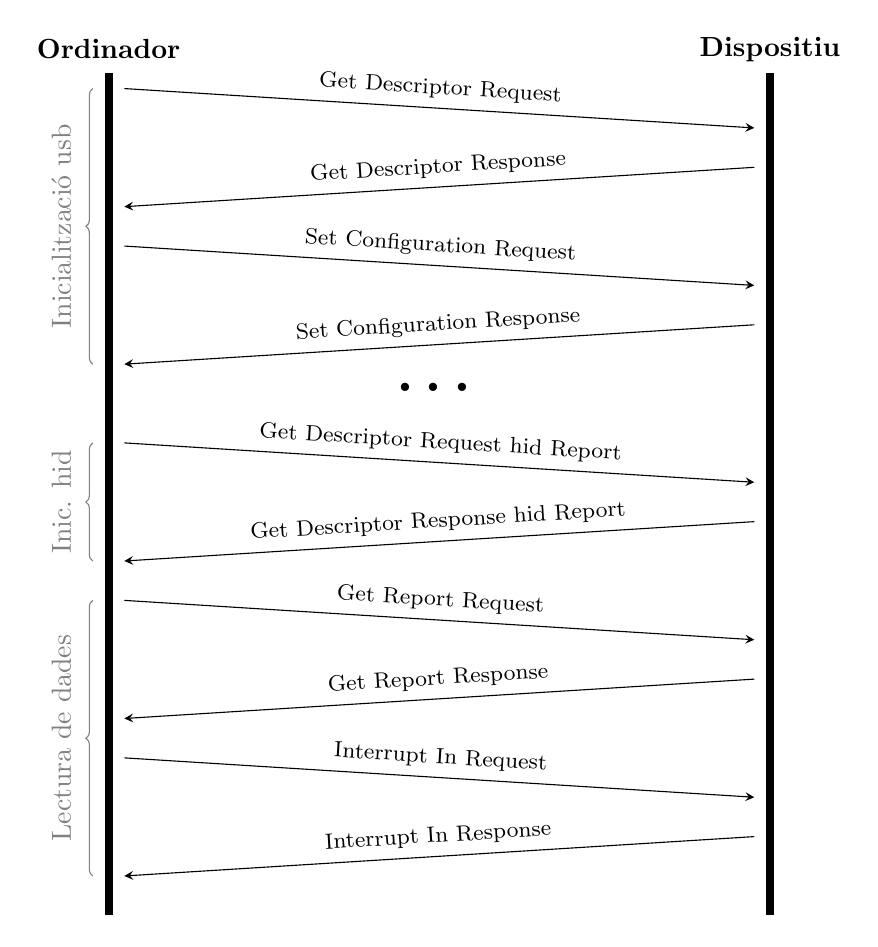
\begin{tikzpicture}[>=stealth]

            \node at (-0.2,0) {\textbf{Ordinador}};
            \node at (8.2,0) {\textbf{Dispositiu}};

            \draw[-] [line width=1mm, black] (-0.2,-0.3) -- (-0.2,-11);
            \draw[-] [line width=1mm, black] (8.2,-0.3) -- (8.2,-11);
        
            % Arrows for packets
            \draw[->] (0,-0.5) -- (8,-1) node[midway, above, sloped] {\footnotesize \acro{Get Descriptor} Request};
            \draw[->] (8,-1.5) -- (0,-2) node[midway, above, sloped] {\footnotesize \acro{Get Descriptor} Response};
            \draw[->] (0,-2.5) -- (8,-3) node[midway, above, sloped] {\footnotesize \acro{Set Configuration} Request};
            \draw[->] (8,-3.5) -- (0,-4) node[midway, above, sloped] {\footnotesize \acro{Set Configuration} Response};
        
            \node at (4, -4.3) {\huge \textbf{\dots}};

            \draw[->] (0,-5) -- (8,-5.5) node[midway, above, sloped] {\footnotesize \acro{Get Descriptor} Request \acro{hid} Report};
            \draw[->] (8,-6) -- (0,-6.5) node[midway, above, sloped] {\footnotesize \acro{Get Descriptor} Response \acro{hid} Report};

            \draw[->] (0,-7) -- (8,-7.5) node[midway, above, sloped] {\footnotesize \acro{Get Report} Request};
            \draw[->] (8,-8) -- (0,-8.5) node[midway, above, sloped] {\footnotesize \acro{Get Report} Response};
            \draw[->] (0,-9) -- (8,-9.5) node[midway, above, sloped] {\footnotesize \acro{Interrupt In} Request};
            \draw[->] (8,-10) -- (0,-10.5) node[midway, above, sloped] {\footnotesize \acro{Interrupt In} Response};

            % Braces
            \draw [decorate, decoration={brace, mirror}, gray] (-0.4,-0.5) -- (-0.4,-4);
            \draw [decorate, decoration={brace, mirror}, gray] (-0.4,-5) -- (-0.4,-6.5);
            \draw [decorate, decoration={brace, mirror}, gray] (-0.4,-7) -- (-0.4,-10.5);

            \node [gray] at (-0.8, -2.25) {\rotatebox{90}{Inicialització \acro{usb}}};
            \node [gray] at (-0.8, -5.75) {\rotatebox{90}{Inic. \acro{hid}}};
            \node [gray] at (-0.8, -8.75) {\rotatebox{90}{Lectura de dades}};

        \end{tikzpicture}
    %\end{adjustbox}

    \caption{Exemple simplificat d'intercanvi de paquets entre un ordinador i un dispositiu \acro{hid}.}
    \label{fig:hid-packets}
\end{figure}


\subsection{Cas concret: acceleròmetre tridimensional}

Tal com es veurà més endavant, s'acabarà utilitzant la categoria de
\est{3D Accelerometer} per designar el tipus de dispositiu. Aquesta
categoria (i la resta de dispositius dins del subgrup de sensors) necessita
reportar un seguit de dades, i no totes són òbvies.

A continuació es detallen les diferents dades que s'han d'enviar. Tal com s'ha
comentat anteriorment, en el \est{\acro{hid} report descriptor} es definirà
el tipus de dispositiu i el format i valors de les dades que s'enviarà, juntament
amb la freqüència amb què l'ordinador les pot so\l.licitar.

\begin{itemize}
    \item En primer lloc, s'ha de comunicar el tipus exacte de dispositiu. En
    aquest cas, la categoria de sensors i el tipus acceleròmetre tridimensional.
    \item S'ha de comunicar el tipus de connexió amb l'ordinador: integrat a
    la mateixa màquina, extern o adjunt. En el cas d'aquest projecte s'utilitzarà
    el tipus \emph{adjunt}, ja que es troba a molta proximitat de l'ordinador
    i en reportarà dades (el tipus extern seria per a sensors que
    mesuren variables d'altres aparells).
    \item També s'han de reportar els esdeveniments que pugui tenir el sensor.
    En aquest cas no se n'ha de reportar cap, així que en aquest paquet
    es definirà solament el tipus genèric \est{No Events}.
    \item L'estat d'alimentació del dispositiu també serà constant per a
    aquest dispositiu (no s'implementarà mode \est{sleep} o de baix consum, i
    la diferència de consum mentre que s'agafen mostres i mentre que
    s'espera una nova lectura de dades és poc significativa). Tanmateix, el
    protocol també ordena enviar-ho de la mateixa forma que la resta d'estats.
    \item El següent valor a enviar és l'estat del sensor. Aquest sí que serà
    diferent en funció de les dades que reporti el sensor. Per exemple, pot
    reportar que hi ha noves dades, que s'està inicialitzant, que hi ha un
    error en la lectura de dades, entre d'altres.
    \item També es reportarà l'interval que proposa el dispositiu entre
    diferents \est{reports}, és a dir, el temps que separarà cada trama de
    tipus \acro{in}.
    \item Finalment, hi ha les dades que es volen enviar. En la capçalera inicial
    s'especificaran moltes configuracions amb relació a les dades: valor màxim,
    mínim, factor d'escala, estat de les dades. Es recomana llegir la
    documentació proposada o veure exemples per entendre la immensitat
    d'aquesta informació.
\end{itemize}

Un cop enviada aquesta capçalera,
l'ordinador podrà demanar tantes vegades com vulgui els valors de les dades, és
a dir, els \est{Reports} definits anteriorment.
Concretament, en el cas d'aquest sensor, l'ordinador podrà demanar dos tipus
de \est{Reports}: \est{feature} i \est{input}.

\begin{itemize}
    \item El tipus \est{feature} enviarà l'estat del sensor: connexió, dades,
    interval entre comunicacions, sensitivitat i esdeveniments.
    \item El tipus \est{input} enviarà l'estat del sensor i, si s'escau, els
    valors llegits. Aquests valors s'hauran de dividir pel factor especificat
    a la capçalera per poder representar decimals. En el cas de l'acceleròmetre,
    la unitat a enviar és $g$, i gairebé mai aquest valor superarà
    les poques unitats; per tant, disposar de decimals és essencial.
\end{itemize}

La tasca que caldrà efectuar quan es dissenyi el programari serà convertir la
informació anterior en el format desitjat per al protocol \acro{hid}. Per sort,
existeixen programes i eines que ajuden a generar aquests codis, tal com
es veurà més endavant.

% Antic subapartat V-USB
\section{Implementacions del protocol USB en AVR}

Un cop es coneix el funcionament del protocol \acro{usb} i se sap quines trames
cal enviar, s'ha d'esbrinar com es pot comunicar un microcontrolador amb
una arquitectura \acro{avr8} amb l'ordinador. En aquest apartat es detallen
les diferents possibilitats que s'han descobert al llarg d'aquest projecte.

\subsection{Perifèrics incorporats}

El primer que s'ha cercat són els microcontroladors amb arquitectura \acro{avr8} que
tinguessin un perifèric \acro{usb} integrat. S'ha trobat la família
\acro{AtMegaXXuX} (en què les X poden ser diferents nombres) de l'empresa
\acro{atmel} \cite{AtMega32u4}. Aquests dispositius, que tenen una \emph{u} en
el seu nom (per remarcar que disposen del perifèric \acro{usb}), permetrien
una comunicació molt senzilla amb l'ordinador.

El dispositiu que més es comentarà durant aquest document és l'\acro{AtMega32u4},
que, en formar part de la placa Arduino Leonardo, és molt fàcil poder fer-hi
proves. També es veurà com s'acaba descartant l'ús de microcontroladors amb
perifèrics incorporats a causa de la diferència de preu en comparació amb les
alternatives següents.

\subsection{Llibreria LUFA}

La llibreria \acro{lufa} és una implementació del protocol \acro{usb} en
programari \cite{Lufa}. Disposa d'una llicència molt permissiva (\acro{mit}) i
funciona amb un gran nombre de dispositius \acro{avr}. De segur que és una
alternativa a tenir present quan s'ha de prendre una decisió com l'actual.

Tanmateix, aquesta llibreria necessita uns perifèrics i maquinari específics
(temporitzadors, freqüència de rellotge, \dots) per funcionar correctament.
Això limita considerablement el nombre de dispositius que es poden triar, ja que
no tots els microcontroladors \acro{avr8} compleixen els requisits que
demana \acro{lufa}. Aquest és el principal motiu pel qual s'acabarà escollint la
darrera opció per al projecte.

\subsection{Llibreria V-USB}

La llibreria \acro{v-usb}, implementada per \est{Objective Development} \cite{Vusb},
implementa la capa més baixa d'\acro{usb} a l'arquitectura
\acro{avr}, sense utilitzar perifèrics específics. Així doncs, gràcies a aquesta
llibreria no serà necessari utilitzar un microcontrolador \acro{avr} dotat amb
perifèrics \acro{usb}, com podria ser, per exemple, l'\acro{AtMega32u4}.

Aquesta llibreria 
es distribueix amb la llicència \acro{gpl-2+}, que obliga a
distribuir sota la mateixa llicència (o versions posteriors) tots els
projectes que facin servir la llibreria. L'empresa ofereix el concepte de
llicència dual: a part de \acro{gpl-2+}, se'n pot comprar una de comercial
per poder generar codi sota altres llicències \cite{VusbLicensing}.

Com que no s'utilitzen perifèrics específics, \acro{v-usb} no pot ca\l.librar amb
precisió el rellotge i els nivells de voltatge per complir el protocol \acro{usb}
amb perfecció. Així doncs, s'ha de tenir present que, per llicenciar un
dispositiu davant d'\acro{usb-if} potser hi haurà alguna complicació més que
habitualment.

A \cite{Vusb} hi ha el codi font de la llibreria, que s'ha d'incloure en el
projecte que s'estigui desenvolupant com a submòdul de \est{git}
\footnote{
    Els submòduls de \est{git}, o \est{Git Submodules}, serveixen per
    situar un repositori de \est{git} en un directori que forma part d'un altre
    repositori de \est{git}. Això permet mantenir els dos projectes separats
    mentre que eines com \est{gcc} poden disposar de l'estructura de
    fitxers necessària \cite{GitSubmodule}.
}, i també s'hi troben exemples de dispositius
senzills (ratolins i teclats) implementats amb aquesta llibreria. Tanmateix,
s'ha trobat el repositori de \cite{VusbProjects} més interessant, ja que conté
exemples de sensors \acro{hid}.

\section{\est{Drivers} a Linux}

Un altre dels aspectes importants del projecte és la creació d'un programari
que pugui fer d'intermediari entre el dispositiu i l'entorn gràfic. Tal com es
mostra en el títol de l'apartat, es comentarà només el cas específic dels sistemes
\acro{unix}, concretament amb Linux, ja que aquest sistema és l'objectiu
principal del projecte.

\subsection{Capes d'abstracció}

El \est{kernel} de Linux acostuma a dividir-ho tot en diferents capes, i no és una
excepció per al que té referència amb aquest projecte. Sempre és recomanable
treballar amb la capa més alta possible, ja que sovint això significa
estalviar-se feina. Tanmateix, és important comprendre d'on es ve per
poder entendre millor els errors i les dificultats que es trobaran en aquest treball.

A la figura \ref{fig:linux-stack} es pot veure una esquematització de la pila
de capes de \est{drivers} que el dispositiu haurà de travessar. Com es pot
veure, la capa més elevada engloba més tipus de dispositius, per la qual cosa aquesta
darrera abstracció aporta molts avantatges a l'hora de fer el programa més
versàtil. Evidentment, l'esquema és una simplificació, ja que darrere de cada
\est{driver} hi ha molta lògica que no hi hauria temps d'explicar en aquest
document.

\begin{figure}[ht]
    \centering

    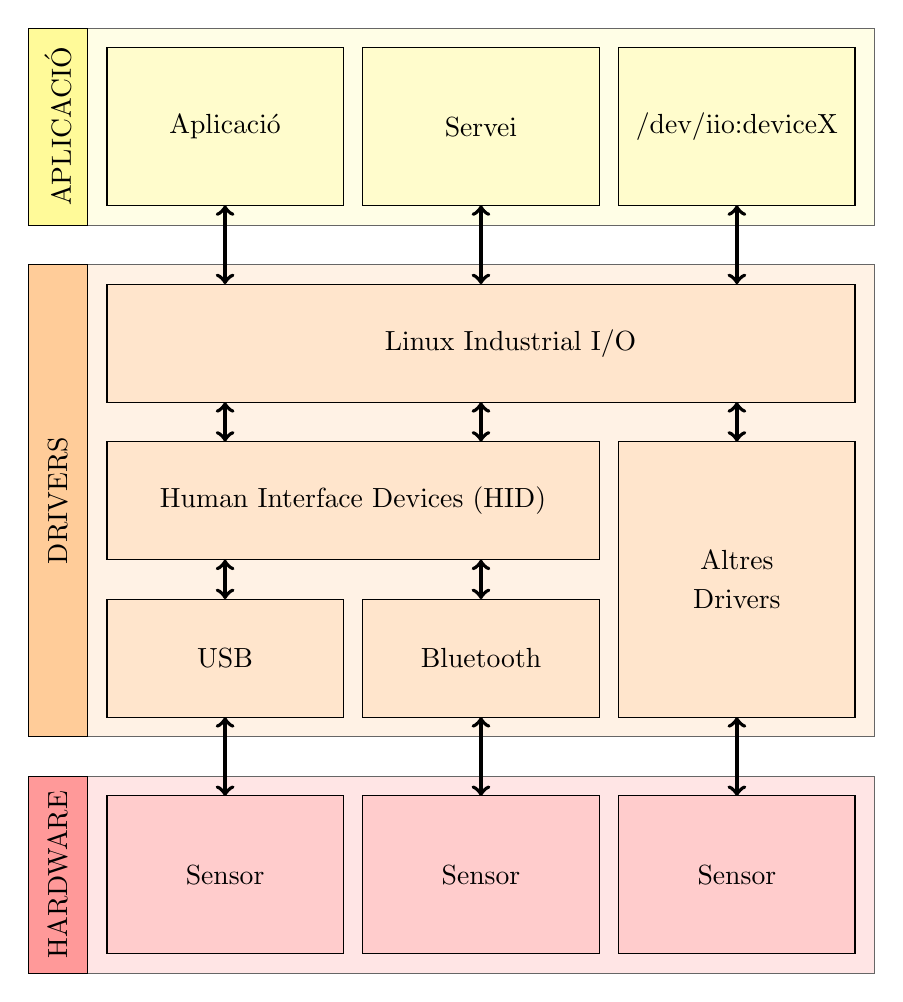
\begin{tikzpicture}
        \filldraw[fill=red!10!white, draw=black!60!white] (0.75,0) rectangle (10.75,2.5);
        \filldraw[fill=orange!10!white, draw=black!60!white] (0.75,3) rectangle (10.75,9);
        \filldraw[fill=yellow!10!white, draw=black!60!white] (0.75,9.5) rectangle (10.75,12);
    
        \filldraw[fill=red!40!white, draw=black] (0,0) rectangle (0.75,2.5);
        \filldraw[fill=orange!40!white, draw=black] (0,3) rectangle (0.75,9);
        \filldraw[fill=yellow!40!white, draw=black] (0,9.5) rectangle (0.75,12);
    
        \node at (0.375,1.25) {\rotatebox{90}{HARDWARE}};
        \node at (0.375,6) {\rotatebox{90}{DRIVERS}};
        \node at (0.375,10.75) {\rotatebox{90}{APLICACIÓ}};
    
        \filldraw[fill=red!20!white, draw=black] (1,0.25) rectangle (4,2.25);
        \node at (2.5,1.25) {Sensor};
        \filldraw[fill=red!20!white, draw=black] (4.25,0.25) rectangle (7.25,2.25);
        \node at (5.75,1.25) {Sensor};
        \filldraw[fill=red!20!white, draw=black] (7.5,0.25) rectangle (10.5,2.25);
        \node at (9,1.25) {Sensor};
    
        \filldraw[fill=orange!20!white, draw=black] (1,3.25) rectangle (4,4.75);
        \node at (2.5,4) {USB};
        \filldraw[fill=orange!20!white, draw=black] (4.25,3.25) rectangle (7.25,4.75);
        \node at (5.75,4) {Bluetooth};
        \filldraw[fill=orange!20!white, draw=black] (1,5.25) rectangle (7.25,6.75);
        \node at (4.125,6) {Human Interface Devices (HID)};
    
        \filldraw[fill=orange!20!white, draw=black] (7.5,3.25) rectangle (10.5,6.75);
        \node at (9,5.25) {Altres};
        \node at (9,4.75) {Drivers};
        \filldraw[fill=orange!20!white, draw=black] (1,7.25) rectangle (10.5,8.75);
        \node at (6.125,8) {Linux Industrial I/O};
    
        \filldraw[fill=yellow!20!white, draw=black] (1,9.75) rectangle (4,11.75);
        \node at (2.5,10.75) {Aplicació};
        \filldraw[fill=yellow!20!white, draw=black] (4.25,9.75) rectangle (7.25,11.75);
        \node at (5.75,10.75) {Servei};
        \filldraw[fill=yellow!20!white, draw=black] (7.5,9.75) rectangle (10.5,11.75);
        \node at (9,10.75) {/dev/iio:deviceX};
    
        \draw[line width=0.5mm, <->] (2.5,2.25) -- (2.5,3.25);
        \draw[line width=0.5mm, <->] (5.75,2.25) -- (5.75,3.25);
        \draw[line width=0.5mm, <->] (9,2.25) -- (9,3.25);
    
        \draw[line width=0.5mm, <->] (2.5,4.75) -- (2.5,5.25);
        \draw[line width=0.5mm, <->] (5.75,4.75) -- (5.75,5.25);
    
        \draw[line width=0.5mm, <->] (2.5,6.75) -- (2.5,7.25);
        \draw[line width=0.5mm, <->] (5.75,6.75) -- (5.75,7.25);
        \draw[line width=0.5mm, <->] (9,6.75) -- (9,7.25);
    
        \draw[line width=0.5mm, <->] (2.5,8.75) -- (2.5,9.75);
        \draw[line width=0.5mm, <->] (5.75,8.75) -- (5.75,9.75);
        \draw[line width=0.5mm, <->] (9,8.75) -- (9,9.75);
    
    \end{tikzpicture}

    \caption{Esquema de les capes d'abstracció per a un dispositiu \est{iio} a Linux.}
    \label{fig:linux-stack}
\end{figure}


\subsubsection*{Capa 1: \est{libusb}}

\est{Libusb} és una llibreria multiplataforma i disponible per a diversos
llenguatges que permet realitzar una comunicació amb dispositius \acro{usb} en
la capa més baixa possible. En aquest nivell es poden enviar trames de control,
entrada o sortida a nivell de bits i bytes \cite{Libusb}.

Tot i que la llibreria es va pensar inicialment per a Linux, sota el nom de
\est{Linux-\acro{Usb}} \cite{LinuxUsb}, s'ha portat a Windows i MacOS,
convertint-la en la millor alternativa per generar programes multiplataforma
que necessitin controladors personalitzats.

Tanmateix, aquest projecte es beneficiarà de les capes de més alt nivell, per la qual cosa
serà més fàcil utilitzar les altres llibreries, tot i que això pugui suposar
efectuar petits canvis entre els diferents sistemes operatius.

A Linux, un dispositiu que es pot controlar per \est{libusb} sol aparèixer com
a fitxer sota el format \fitx{/dev/usbrawX}, en què X és el número de dispositiu.
No gens menys, si un controlador d'una capa superior està utilitzant
exclusivament el dispositiu, el \est{kernel} no crearà aquest fitxer, per
evitar confusió i solapaments.

\subsubsection*{Capa 2: \est{libhid} i \est{hidapi}}

La següent llibreria és la capa immediatament superior a la de l'apartat
anterior. \est{Libhid} permet gestionar dispositius \acro{hid}. D'aquesta
llibreria ha nascut \est{hidapi}, que l'engloba i la converteix en
una abstracció compatible amb altres sistemes operatius, com
FreeBSD, Windows i MacOS \cite{Libhid}. Tal com s'ha dit a 
l'apartat \ref{sec:hut}, també permetrà utilitzar dispositius Bluetooth.

Com que aquesta llibreria és una abstracció més elevada, existeixen més aplicacions
per provar-la i depurar-la. Sobretot es destaca \cite{LibhidUI}, que disposa
d'una interfície molt senzilla d'utilitzar i multiplataforma.

A Linux, un dispositiu que es pot controlar per \est{libhid} sol aparèixer com
a fitxer sota el format \fitx{/dev/hidrawX}, en què X és el número de dispositiu.
De la mateixa forma que amb l'apartat anterior, el dispositiu no apareixerà
sota aquest format si una capa més alta l'està utilitzant exclusivament.

\subsubsection*{Capa 3: \est{libiio}}

Finalment, la darrera capa d'abstracció de la pila d'aquest projecte és la
llibreria \acro{libiio}.
Aquesta llibreria permet interaccionar amb el sistema
\acro{iio} de Linux. També està disponible per a diversos llenguatges, però
a diferència de la resta d'abstraccions, no és multiplataforma.

El sistema \acro{iio}, o \est{Industrial Input/Output}, és la capa d'abstracció
dels sistemes basats en Linux per a qualsevol dispositiu que suposi una entrada
o sortida per al sistema i no tingui controladors dedicats. Per exemple, un
ratolí o un teclat no entraria dins d'aquest grup, ja que disposa de controladors
propis \cite{Iio}.

Hi ha moltes formes de veure quines categories de dispositius \acro{hid} es
converteixen en \acro{iio}, però la més senzilla és consultant el codi
font de Linux \cite{KernelIioAccel}. Pel que fa a aquest projecte, es pot veure
que existeix un \est{driver} per a \est{hid\_accelerometer\_3d} i, per tant, el
dispositiu d'aquest treball anirà en aquesta capa superior.

Mitjançant normes \acro{udev} es podria aconseguir que un dispositiu que per 
defecte s'assigna a \acro{iio} es quedi una capa més per sota, com seria
\acro{hid} o \acro{usb}. Tanmateix, \acro{iio} aporta molts beneficis.

\begin{itemize}
    \item No necessita permisos suplementaris per llegir les dades dels
    sensors. Per tant, no s'ha d'afegir l'usuari en un grup nou ni crear
    cap regla \acro{udev}.
    \item Més d'un usuari o procés pot estar llegint simultàniament el sensor.
    El dispositiu creat a \fitx{/dev/iio:deviceX} (en què X és el número de
    dispositiu) pot ser llegit simultàniament, de la mateixa forma que ho fan
    altres fitxers, per exemple \fitx{/dev/rand} o \fitx{/dev/zero}.
    \item En ser una capa superior, no s'ha de gestionar tot el referent al
    protocol \acro{hid}. Les lectures del sensor venen gairebé completament
    processades.
    \item Finalment, en ser una capa superior, també hi tenen cabuda altres
    sensors que podrien servir per al projecte, però que no són \acro{hid}.
\end{itemize}

Així doncs, es pagarà el preu de generar programari no compatible amb altres
dispositius a canvi de generar programari robust i a la capa més alta possible
per Linux. Pot semblar una mala decisió, però es veurà en el següent apartat
que tampoc seria possible generar un controlador 100 \% multiplataforma.

\subsection{Gestió i assignació de dispositius}

Un sistema operatiu amb tantes capes d'abstracció necessita forçosament una
aplicació que gestioni quina preval i quins usuaris hi poden accedir.
\acro{Udev} és el gestor de dispositius per a sistemes basats en Linux.
Té com a objectiu gestionar dinàmicament els dispositius de maquinari del
sistema, és a dir, és el responsable que si es connecta o desconnecta
un dispositiu mentre l'ordinador està encès, tot funcioni amb normalitat \cite{Udev}.

El funcionament d'\acro{udev} es basa en un conjunt de regles,
que es configuren per
determinar com han de gestionar-se els dispositius detectats.
Aquestes regles es poden configurar i modificar i, en el cas d'aquest projecte,
s'utilitzaran exclusivament per permetre a tots els usuaris utilitzar alguns
dispositius concrets, siguin quins siguin els permisos. Tanmateix, \acro{udev}
ofereix molta flexibilitat: es poden executar \est{scripts}, canviar el nom,
crear un volum, entre moltes altres possibilitats.

Com és d'esperar, només un usuari amb permisos d'administrador podrà configurar
les regles \acro{udev}, i hi ha molts paràmetres per configurar al màxim
aquestes regles. Tanmateix, com que aquestes normes només seran d'utilitat durant
el procés de desenvolupament del dispositiu, s'ha decidit no entrar gaire en
detalls de la implementació.

\subsubsection*{Exemples d'ús d'UDEV}

Un clàssic cas d'ús d'\acro{udev} és quan es vol que un dispositiu \acro{usb}
concret (identificat a través de la parella de codis \acro{vid}-\acro{pid})
sigui accessible per a un usuari concret. Això és necessari, per exemple, per
poder programar una placa Arduino o similar sense haver d'utilitzar permisos
d'administrador cada vegada.
Tot i que en aquest exemple la solució més encertada seria afegir l'usuari
corresponent al grup \fitx{dialout}, també es pot assolir l'objectiu proposat
afegint una regla \acro{udev}.

El següent fitxer, anomenat \fitx{49-micronucleus.rules}, permet programar una
placa \est{Digispark} mitjançant l'ordre \ord|micronucleus|. El nom del fitxer
comença amb un nombre per un motiu concret: el \est{kernel} carregarà totes les
regles que hi hagi a \fitx{/etc/udev/rules.d/} en ordre alfabètic dels fitxers.
A partir d'aquest requisit s'ha creat una convenció per utilitzar dos nombres
per ordenar aquests fitxers \cite{Udev}.

A continuació es mostra el contingut del fitxer
\footnote{
    Les regles \acro{udev} no poden tenir salts de línia. Per facilitar la
    lectura s'ha utilitzat la contrabarra per representar les regles en
    diferents línies, però copiades literalment donarien en un error.
}:

\begin{verbatim}
SUBSYSTEMS=="usb", ATTRS{idVendor}=="16d0", ATTRS{idProduct}=="0753", \
                   MODE:="0666"
KERNEL=="ttyACM*", ATTRS{idVendor}=="16d0", ATTRS{idProduct}=="0753", \
                   MODE:="0666", ENV{ID_MM_DEVICE_IGNORE}="1"
\end{verbatim}

Com es pot veure, hi ha dues regles:
\begin{itemize}
    \item La primera donarà accés a tots els usuaris (posant el mode
    \texttt{0666}) a tots els dispositius que utilitzin el \est{driver}
    \texttt{usb} i que tinguin el \acro{vid} i \acro{pid} assenyalats.
    \item La segona realitza el mateix, però amb aquells que utilitzin el
    \est{driver} \texttt{ttyACM} (dispositius de comunicació). També evita que
    el \est{driver} del mòdem (\est{ModemManager}) prengui control del
    dispositiu fent que l'ignori.
\end{itemize}

\subsubsection*{Assignar \est{drivers} específics}

Com s'ha vist a l'exemple anterior, és possible crear regles \acro{udev} per
canviar el \est{driver} o controlador d'un dispositiu. També es poden desvincular
controladors mitjançant l'ordre \ord|udevadm|, que, com que no modifica cap fitxer
a \fitx{/etc}, no és persistent.

Així doncs, gràcies a aquesta ordre o a la configuració de regles \acro{udev},
es pot evitar que un dispositiu utilitzi un \est{driver} d'una capa superior.
És possible, doncs, mostrar un fitxer \fitx{/dev/usbrawX} d'un dispositiu
\acro{hid} \cite{unbindingHid}, tot i que per defecte aquests utilitzin
\fitx{libhid} i no \fitx{libusb}.

\section{Execució en segon pla a Linux}
\label{subsec:systemd}

El programari que es pretén realitzar per a aquest projecte involucra la
presència d'un procés que, en tot moment, comprovi les lectures del sensor i
actualitzi l'orientació de la pantalla. L'usuari és responsable d'insta\l.lar i
configurar el programa, però un cop configurat, aquest hauria de funcionar
sempre correctament, fins i tot després de reiniciar l'ordinador.

En els sistemes basats en Linux, els programes que estan en execució tota
l'estona s'anomenen serveis i els gestiona el propi \est{kernel}, també anomenat,
en aquest context, \est{systemd} \cite{Systemd}. Hi ha dos tipus de serveis
diferents, en funció dels privilegis que tenen:

\begin{itemize}
    \item Els \emph{serveis del sistema} afecten a tots els usuaris i
    s'executen sota l'usuari i context de \est{root} (excepte si es diu
    el contrari). Es pot escollir quan s'executen, ja sigui just després de
    carregar el \est{kernel} a la memòria o després que el primer usuari
    iniciï sessió. Es necessiten permisos d'administrador per fer modificacions
    en els serveis de sistema (generalment mitjançant l'ordre \ord|systemctl|).
    \item Els \emph{serveis d'usuari}, en canvi, només afecten l'usurari
    que els ha configurat. No es necessiten permisos d'administrador per
    configurar-los, i s'executen sota el mateix context, variables d'entorn i
    usuari que qui els ha configurat. Aquests serveis només es poden executar a
    partir dels darrers passos de l'arrencada del sistema, ja sigui després
    d'iniciar sessió o un cop carregat l'entorn gràfic. També utilitzen l'ordre
    \ord|systemctl|, però afegint l'opció \ord|--user|.
\end{itemize}

És important conèixer la diferència entre els dos tipus mencionats, ja que en
aquest treball es generarà un servei d'usuari i un de sistema, i cadascun té
les seves complicacions, tant en el moment d'insta\l.lació com en el moment
d'execució.

\section{Entorn gràfic a Linux}

El darrer punt a tractar en aquest capítol és la comunicació entre una
aplicació i l'entorn gràfic en un sistema basat en Linux; concretament, cal
esbrinar com aplicar canvis de rotació de la pantalla. Per sort, 
independentment de l'entorn gràfic que utilitzi un ordinador (normalment
\acro{gnome}, però també \acro{kde}), tots responen a les peticions gràfiques
sota la interfície de programació de \est{Xlib} \cite{Xlib}.

Es podria fer una bona analogia entre
els entorns gràfics i els navegadors: els navegadors, a Linux, implementen les
crides i interfície de \est{www-browser}, tot i estar implementats internament
de formes diferents. Si es vol implementar una aplicació que necessiti, per
exemple, un navegador incrustat, però qualsevol navegador serveix, es pot
indicar com a dependència \est{www-browser} en lloc de, per exemple, \est{Firefox}.

\subsection{Servidor gràfic \est{Xorg}}

\est{Xorg} és un servidor gràfic per gestionar des de configuracions de
pantalla fins a detalls de rendiment per a certes finestres. Els programes
utilitzen la llibreria \est{Xlib} per interactuar-hi.
\est{Xlib} és una llibreria molt complexa, i té interfícies per a la majoria
dels llenguatges.

Tanmateix, sovint és més senzill utilitzar una aplicació de
la línia d'ordres que simplifica la tasca del programador. Aquesta
aplicació es diu \est{xrandr} i, d'una forma molt senzilla, permet llistar
totes les pantalles connectades a l'ordinador i canviar l'orientació
d'una d'elles \cite{Xrandr}.

A la figura \ref{fig:xorg-hyerarchy} es pot contemplar la jerarquia de la qual
es parla: \est{xrandr} segueix sent un intermediari més entre l'aplicació que
es vol crear i l'objectiu final: rotar la pantalla. De nou, en treballar amb
diverses capes torna a aparèixer la possibilitat d'utilitzar un programa
diferent per a les capes superiors: per exemple, \est{xrandr} pot ser utilitzat
des de la línia d'odres, a part de des de l'aplicació que es dissenyi.

\begin{figure}[ht]
    \centering
    % \begin{forest}
    %     forked edges,
    %     for tree={draw,align=center,edge={-latex}}
    %     [\est{Xorg}
    %         [\est{Xlib}
    %             [\texttt{xrandr}
    %                 [Aplicació]
    %             ]
    %         ]
    %     ]
    % \end{forest}

    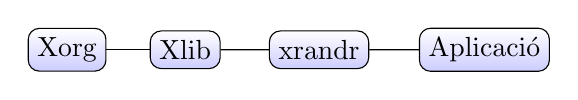
\begin{tikzpicture}[
        grow = right,
        every node/.style = {shape=rectangle, rounded corners,
          draw, align=center,
          top color=white, bottom color=blue!20}]
        \node {\est{Xorg}}
            child {
                node {\est{Xlib}} 
                child {
                    node [xshift=0.2cm] {\est{xrandr}}
                    child {
                        node [xshift=0.6cm] {Aplicació}
                    }
                }
            };
    \end{tikzpicture}

    \caption{Intermediaris entre \est{Xorg} i l'aplicació final \cite{Xrandr}.}
    \label{fig:xorg-hyerarchy}
\end{figure}


\subsection{Execució de \est{Xrandr} en un servei de sistema}
\label{subsec:xrandr}

Els sistemes Linux estan construïts per ser tan versàtils com sigui possible. Una
de les possibilitats és que hi hagi diferents clients connectats a la vegada
a la mateixa màquina. Aquest fet no sorprèn a ningú, ja que és ben sabut que
diversos usuaris poden connectar-se remotament i simultàniament a la mateixa
màquina mitjançant \est{ssh}. Ara bé, hi ha diverses formes (com, per exemple,
l'opció \ord|-X| de \est{ssh}) que permeten diferents sessions gràfiques
simultàniament \cite{ManSSH}.

La complicació rau en el fet que \est{xrandr} utilitza les variables d'entorn per
trobar la sessió actual. Aquestes variables es defineixen a l'inici de sessió,
quan s'inicialitza \est{Xlib}. Això vol dir que, sempre que s'executi
\est{xrandr} des de la sessió (ja sigui amb un servei de sessió o a través de
la línia d'odres) no hi haurà cap problema.
Tanmateix, si es vol executar \est{xrandr} des d'un servei de sistema o des d'un
terminal remot, el programa no trobarà la sessió actual i serà impossible
resoldre la comanda \cite{ArchWiki}.

Hi ha entre dos i tres variables d'entorn importants per al correcte funcionament
de \est{xrandr} \cite{XrandrVars}:

\begin{itemize}
    \item La variable d'entorn \verb|$DISPLAY| permet identificar el grup de
    pantalles al qual s'està connectat. En general sempre serà \verb|:0| (o 
    \verb|:1| pels sistemes més recents), però si hi ha diversos usuaris
    connectats amb diferents entorns gràfics, podria ser un altre nombre.
    \item La segona variable d'entorn necessària és \verb|$XAUTHORITY|. Aquesta
    variable conté la direcció del fitxer \fitx{Xauthority}. Aquest fitxer
    conté la \est{cookie} o galeta que permet consultar i realitzar canvis en la sessió
    actual. Com és evident, aquest fitxer només pot ser consultat per l'usuari
    propietari de la sessió (i usuaris administradors).
    \item Finalment, hi ha \verb|$XDG_RUNTIME_DIR|, que pretén reemplaçar la
    variable anterior per portar la direcció del directori que conté el fitxer
    \est{Xauthority}.
\end{itemize}

Cal tenir present que un usuari pot restringir qui té accés a modificar la
seva sessió. Per defecte, es restringeix a tothom que no tingui accés al
fitxer d'autorització, però mitjançant l'ordre \ord|xhost +| es pot permetre
que tothom pugui efectuar modificacions a la sessió d'aquell usuari \cite{Xhost}.
Tanmateix, aquesta pràctica es considera poc segura, i per aquest motiu no es
tindrà en compte durant l'elaboració d'aquest treball.

%\subsection{Linux i els controladors gràfics}
%TODO Restructurar o col·locar en un altre lloc "Experiències personals"

% Qualsevol persona que hagi provat d'insta\l.lar els controladors oficials
% d'una targeta gràfica en un entorn Linux sabrà que no és pas cap tasca trivial.
% Tot i haver millorat recentment, hi segueixen havent moltes incompatibilitats
% entre diferents versions i targetes gràfiques. En el cas concret d'aquest
% projecte s'ha utilitzat un ordinador equipat amb una \acro{nvidia gtx1050},
% un model utilitzat en molts dispositius.

% Tanmateix, en el moment de provar l'ordre \ord|xrandr| es va descobrir que,
% en funció dels controladors de la targeta gràfica que hi hagi activats a
% l'ordinador i de les seves versions, l'execució de l'ordre causa un congelament
% de mig segon aproximadament de totes les pantalles del sistema. Aquest error ja
% ha estat reportat a \cite{xrandrBug}, però no s'ha trobat cap solució
% específica.

% S'ha solucionat aquest problema desinsta\l.lant els controladors gràfics de
% \acro{nvidia}. Tanmateix, això deixava inutilitzable la connexió \acro{hdmi} de
% l'ordinador. Finalment, es va optar per actualitzar la distribució d'Ubuntu
% (de 18.04 a 24.04) on aquest error ja no ha tornat a aparèixer (n'han aparegut
% d'altres, però no han afectat pel desenvolupament d'aquest projecte).

\subsection{Transició al servidor gràfic \est{Wayland}}
\label{subsec:wayland}

El servidor gràfic de l'apartat anterior, \est{Xorg}, és un projecte molt antic
i porta acumulades bastants funcionalitats i canvis que s'ha fet durant els
anys. Si bé és molt funcional i popular, es podria crear un entorn gràfic que
funcionés d'una forma més eficient amb el maquinari actual (el \est{hardware}
ha canviat molt des dels seus inicis). Aquesta és la idea que van tenir les
persones que van impulsar \est{Wayland}.

Creat l'any 2008, ha anat recuperant totes les funcionalitats de \est{Xorg}
implementades amb una arquitectura bastant diferent. Tot i seguir sent
compatible amb alguns aspectes senzills, hi ha molts programes que deixen de
funcionar amb aquest nou servidor, especialment els que comparteixen pantalla
o hi interactuen. Des d'Ubuntu 17.10 que el sistema operatiu deixa
escollir entre els dos entorns \cite{Wayland}.

Tanmateix, un canvi d'aquesta magnitud no es fa d'una versió per una altra.
\est{Wayland} encara necessita bastants millores per fer-lo completament
compatible; per això, la seva \acro{api} no és del tot definitiva. Es preveuen
encara uns quants anys fins que no s'anunciï la data en què \est{Xorg} haurà de
deixar de ser utilitzat; i un cop passada aquesta data, el més probable és que
ordres com \ord|xrandr| segueixin funcionant, de la mateixa forma que segueixen
funcionant eines com \ord|ifconfig|, obsoletes des de fa ja molts anys
\cite{Ifconfig}.

Per aquest motiu s'ha decidit realitzar el projecte utilitzant \est{Xorg}.
D'aquesta forma s'obtindrà un programari estable, si més no durant els primers
anys. Així doncs, si el projecte té previsió de continuar més enllà d'aquest
Treball de Fi de Grau, s'haurà de preveure una migració a \est{Wayland}.

\chapter{Disseny del \est{hardware}}

En aquest capítol es detallarà tot el procés de realització del maquinari per
al projecte. La base teòrica del capítol anterior pot resultar de gran utilitat
per entendre certes decisions preses durant algunes de les tasques d'aquest
capítol.

En aquest projecte es vol obtenir una placa de circuit imprès que permeti
transferir dades d'un sensor d'acceleració a l'ordinador, mitjançant la connexió
\acro{usb}. S'enviarà a producció la placa i es crearà un encapsulat senzill per
evitar que s'ompli de pols o d'altres elements de l'entorn.
Finalment, es llicenciarà el disseny davant d'una entitat certificadora.

\section{Selecció del sensor}
\label{sec:sensor_selection}

El primer pas per crear la placa és escollir quin sensor utilitzar. Per
mesurar la inclinació d'un dispositiu se sol utilitzar un acceleròmetre.
Mitjançant un càlcul que es veurà més endavant i donades unes certes condicions, 
es pot determinar l'angle amb relació a la direcció de la gravetat de la Terra
\cite{PedleyTilt}.
Aquestes mesures es poden complementar amb un giroscopi, que ofereix més
precisió al sistema \cite{6702711}.

Després de fer una mica de recerca sobre els productes disponibles del mercat
i tenint present la precisió que es necessita i el pressupost que es disposa,
s'han trobat dues alternatives viables.

\begin{itemize}
    \item Els sensors \est{ADXL3xx} es poden trobar a preus molt llaminers i
    comuniquen la lectura de l'acceleració en tres dimensions mitjançant tres 
    línies analògiques. Per tant, la comunicació amb el microcontrolador serà la 
    més senzilla possible \cite{adxl335}.
    \item El sensor \est{MPU6050}, en canvi, es comunica amb el microcontrolador
    mitjançant el protocol \acro{i2c}. Aquest protocol només necessita dues
    línies de comunicació, però implica implementar una mica de lògica per
    recuperar les dades. Tanmateix, aquest sensor també ofereix lectures de
    velocitat angular i temperatura, que podrien ser útils per a futures
    millores del projecte \cite{mpu6050specs}.
\end{itemize}

Així doncs, com que el segon sensor és només pocs cèntims més car i ofereix
la possibilitat d'ampliar el projecte en un futur, s'utilitzarà el sensor
\est{MPU6050} per al sistema.

Aquest sensor se sol vendre amb una placa que estalvia connectar
certa electrònica i que permet provar el sensor sense fer cap soldadura.
Aquest mòdul, anomenat \est{GY521}, es troba disponible a moltes botigues
d'electrònica, i s'ha decidit adquirir-ne un parell per al desenvolupament del
projecte. A la figura \ref{fig:gy521img} es pot veure l'aspecte d'aquest mòdul.

\begin{figure}[ht]
    \centering
    \includegraphics[width=0.3\textwidth]{images/modules/gy521img.jpg}
    \caption{Mòdul \est{GY521} \cite{gy521}.}
    \label{fig:gy521img}
\end{figure}

El circuit del mòdul \est{GY521} és lliure i es pot consultar a la figura
\ref{fig:gy521sch}. És prou senzill diferenciar la part utilitzada per
convertir els 5 V d'entrada en 3.3 V per alimentar l'integrat de la resta
del circuit. Aquest mòdul també inclou un \acro{led} per indicar que s'està
alimentant correctament.

Les connexions del lateral del mòdul fan molt còmode utilitzar-lo en entorns de
desenvolupament, on es connecten i desconnecten cables constantment. El fet
de disposar també d'un sistema funcional des d'un primer moment ajuda a
centrar-se només en la part de més alt nivell: l'aplicació del projecte.

\begin{figure}[ht]
    \centering
    \includegraphics[width=0.6\textwidth]{images/modules/gy521sch.png}
    \caption{Esquema elèctric del mòdul \est{GY521} \cite{gy521}.}
    \label{fig:gy521sch}
\end{figure}

\section{Primera versió de la placa}

En un primer moment es va decidir utilitzar un microcontrolador que disposés
del perifèric \acro{usb} directament al maquinari, per evitar programar-lo tot.
Tanmateix, es veurà que no s'acabarà utilitzant aquesta versió a causa de motius
que s'explicaran més endavant. Dit això, s'ha decidit conservar aquest apartat
per comprendre millor el procés de desenvolupament del projecte.

El microcontrolador que s'utilitzarà en aquesta versió és l'\acro{AtMega32u4}, 
que proporciona una interfície \acro{usb} integrada i permet utilitzar-la
\acro{i2c} amb suficient facilitat. S'ha decidit utilitzar un osci\l.lador 
extern per generar un rellotge de freqüència
\SI[round-mode=places,round-precision=0]{16}{\mega\hertz}
al microcontrolador \cite{AtMega32u4}.

\subsection{Esquemàtic}

El disseny de l'esquemàtic es basa en el disseny del mòdul \est{GY521} i es pot
consultar a la figura \ref{fig:sch_v1}. Tret del que s'ha comentat en els paràgrafs
anteriors, la resta de components i connexions no deixen de ser les evidents per
a un circuit amb aquestes característiques. Tot i això, s'ha decidit posar
èmfasi en alguns detalls en què s'ha parat més atenció:

\begin{figure}[ht]
    \centering
    \includegraphics[width=0.9\textwidth]{images/kicad/gyro1_sch.png}
    \caption{Esquema elèctric de la primera versió.}
    \label{fig:sch_v1}
\end{figure}

\begin{itemize}
    \item Al costat de l'alimentació de cada integrat s'hi ha posat un
    condensador ceràmic de
    \SI[round-mode=places,round-precision=0]{10}{\micro\farad} o
    \SI[round-mode=places,round-precision=1]{0.1}{\micro\farad}
    (en funció del que recomanava
    cada fabricant al seu \est{datasheet}), per assegurar-se que la tensió
    d'entrada és prou estable.
    \item S'ha hagut de posar un regulador lineal en el circuit, ja que el
    sensor necessita estar alimentat a
    \SI[round-mode=places,round-precision=1]{3.3}{\volt},
    però l'alimentació que proporciona
    el connector \acro{usb} és de \SI[round-mode=places,round-precision=0]{5}{\volt}.
    \item En utilitzar un connector de tipus C, tot i comunicar-se amb
    \acro{usb2}, hi ha un parell de cables extres que determinen a quina tensió
    s'ha d'alimentar el dispositiu. Tal com es comenta a \cite{Axelson2015USB}
    o a \cite{TypeCIntro}, si es vol utilitzar una alimentació tradicional de 
    \SI[round-mode=places,round-precision=0]{5}{\volt}, és suficient
    utilitzar dos \est{pull-downs} de
    \SI[round-mode=places,round-precision=1]{5.1}{\kilo\ohm}.
    \item El protocol \acro{i2c} necessita que les dues línies de comunicació
    estiguin amb \est{pull-ups}. Més endavant es veurà el funcionament d'aquest
    protocol.
    \item L'esquema referent al cristall extern per al rellotge del microcontrolador
    és el recomanat pel fabricant en el mateix \est{datasheet} \cite{AtMega32u4}.
\end{itemize}

Cal destacar que, a diferència de la propera versió, aquest esquema sí que preveu
una connexió \acro{isp} per programar la placa i un \acro{led} i polsador per
interactuar d'una forma senzilla.

\subsection{Placa de circuit imprès}

Un cop acabat el disseny, utilitzant també el programa KiCad, es va començar a
crear la placa de circuit imprès. El procediment és prou senzill i se sol fer
de forma iterativa: crear un disseny molt dolent i anar-hi fent millores, fins
al punt en què es considera que ja està prou bé (un disseny mai estarà perfecte).

A la figura \ref{fig:pcb_v1} es pot consultar la placa resultant. Com es pot veure,
no està ben distribuïda del tot: això es deu al fet que es va decidir canviar 
completament de disseny abans d'haver-la acabat, i es va pensar que no valia la 
pena seguir invertint temps amb un disseny que no veuria mai la llum.

\begin{figure}[ht]
    \centering
    \includegraphics[width=0.8\textwidth]{images/kicad/gyro1_pcb.png}
    \caption{Placa de circuit imprès de la primera versió.}
    \label{fig:pcb_v1}
\end{figure}

\subsection{Problemes del primer disseny}

Tal com s'ha dit a l'apartat anterior, no es va acabar de dissenyar la placa
de circuit imprès a causa del redisseny del \est{hardware}. El motiu és ben senzill,
no s'està utilitzant el microcontrolador adequat per al projecte.

Tal com s'ha vist a l'esquemàtic, el microcontrolador només necessita quatre potes
per a informació (dos per \acro{usb} i dos per \acro{i2c}). Això significa que es
deixaran al voltant de vint entrades sense utilitzar. I no només això: aquest
microcontrolador disposa de molta més memòria de la que mai es necessitarà
\cite{AtMega32u4}.

El principal motiu per fer el canvi és, doncs, el preu \cite{AvrComparison}.
Un \acro{AtMega32u4} no és gaire car (val \SI{4.92}{\EUR} a Mouser, si es compra
únicament una unitat), però és més barat un dispositiu \acro{avr} de la sèrie
\acro{AtTinyXX} (el model \acro{AtTiny85} val \SI{1.54}{\EUR} a la mateixa
botiga que abans), com es veurà en el següent apartat.

\section{Segona versió de la placa}

Tal com s'ha comentat al final de l'apartat anterior, s'ha decidit apostar
per un microcontrolador més econòmic i senzill atesos els pocs requisits que
demana el sistema. Després de fer una mica de recerca, s'ha descobert la
família de microcontroladors \acro{AtTinyX5}, en què la X pot variar en funció de
la memòria \est{flash} disponible \cite{AtTiny85}.

Aquests microcontroladors disposen de vuit potes, de les quals dos són per a
l'alimentació. Així doncs, de les sis potes disponibles, encara en sobraran dues
per si es vol afegir algun perifèric extra. Per a aquesta versió del projecte,
però, s'ha decidit no donar-hi cap ús.

Tanmateix, abans de produir una placa de circuit imprès, hi havia interès en
poder provar el microcontrolador per assegurar-se que seria possible
realitzar el sistema amb aquest darrer. A través de recerca i recomanacions del
personal del laboratori de l'escola, es va prendre coneixement de l'existència de
la placa \est{Digispark}.

\subsection{Proves prèvies amb la placa \est{Digispark}}
\label{subsec:hw_digispark}

La placa \est{Digispark} es pot comprar a preus molt reduïts (sovint a menys de 
\SI[round-mode=places,round-precision=0]{8}{\EUR}) i a molts llocs.
És una placa de circuit imprès equipada d'un \acro{AtTiny85}, un connector
\acro{usb}, algun component per regular les tensions, i tot de pins per
poder connectar fàcilment qualsevol cable i component al microcontrolador
\cite{Digispark}. A la figura \ref{fig:digispark} es pot veure l'aspecte físic
de la placa.

\begin{figure}[ht]
    \centering
    \includegraphics[width=0.3\textwidth]{images/modules/digisparkimg.png}
    \caption{Placa \est{Digispark} \cite{Digispark}.}
    \label{fig:digispark}
\end{figure}

Aquesta placa és de maquinari obert i, per tant, el seu esquema elèctric també 
es pot trobar fàcilment. A la Figura \ref{fig:digisparksch} es pot veure que
el circuit és prou senzill i només hi ha un parell de detalls que mereixen
la seva explicació, com podria ser l'ús de Díodes Zener. Es comentarà en el
moment del disseny del mateix circuit.

\begin{figure}[ht]
    \centering
    \includegraphics[width=0.8\textwidth]{images/modules/digisparksch.jpg}
    \caption{Diagrama de la placa \est{Digispark} \cite{Digispark}.}
    \label{fig:digisparksch}
\end{figure}

El microcontrolador ve programat amb un \est{bootloader} que utilitza la
llibreria \acro{v-usb} per identificar-se com un port sèrie a l'ordinador
(és una de les subclasses \acro{hid}) i així poder programar-lo fàcilment.
És una placa bastant popular, de maquinari obert i amb molta documentació i
tutorials disponibles per internet \cite{DigisparkBootloader}.

Es va adquirir un parell d'unitats d'aquesta placa i es va connectar amb el
mòdul del sensor d'acceleració. Mitjançant tutorials, utilitzar la placa
\est{Digispark}  era igual de senzill que si es tractés d'un Arduino. Es podia, 
per exemple, utilitzar la llibreria \est{LittleWire} per comunicar-se amb el sensor
amb el protocol \acro{i2c} i llegir les dades necessàries.

Durant el transcurs d'aquestes proves també es va descobrir el projecte
\est{i2c\_tiny\_usb}, que va donar unes conclusions molt interessants. Es
comentaran els resultats amb més detall a l'apartat \ref{sec:testinc-i2c-tiny}.

Així doncs, s'ha acabat utilitzant la placa \est{Digispark} per validar
que el projecte es podria desenvolupar en aquest maquinari i, un cop es va
conèixer la bona notícia, es va començar a desenvolupar la pròpia placa de circuit
imprès.

\subsection{Esquemàtic}

L'esquemàtic d'aquesta segona versió no té gaires secrets. Consisteix a agafar
el circuit de la versió anterior i canviar tot el que té a veure amb l'antic
microcontrolador per al nou. S'ha utilitzat com a referència el circuit de la
placa \est{Digispark}, tenint en compte que algunes coses, com el regulador de
tensió extern, no són necessàries per a aquest projecte \cite{Digispark}.

En aquest nou circuit s'utilitza el rellotge intern del microcontrolador, que
ja s'ha vist que és suficient per comunicar-se per \acro{usb}. Només hi ha
una novetat a comentar en aquesta segona versió, i és la presència de dos
díodes Zener en les línies d'\acro{usb}. El motiu rau en el protocol \acro{usb}:
tot i estar alimentat a \SI[round-mode=places,round-precision=0]{5}{\volt},
les línies de dades funcionen a
\SI[round-mode=places,round-precision=1]{3.3}{\volt}. Tal com
s'ha comentat a l'apartat \ref{subsub:usb_physic}, els dos díodes asseguren
que la tensió no supera mai aquest llindar.

\begin{figure}[ht]
    \centering
    \includegraphics[width=1\textwidth]{images/kicad/gyro2_sch.png}
    \caption{Esquema elèctric de la segona versió.}
    \label{fig:sch_v2}
\end{figure}

Finalment, s'observa que en el diagrama de la figura \ref{fig:sch_v2}
no hi ha cap element amb el qual una
persona pugui interactuar directament amb el dispositiu (polsador, llum, \dots).
Això és a propòsit, ja que es pretén que el dispositiu acabi tancat en una capsa
i que l'usuari no hagi de tocar-lo mai.

\subsection{Placa de circuit imprès}

Un cop creat l'esquema elèctric, s'ha pogut començar a dissenyar la placa de
circuit imprès, de la mateixa manera que amb la versió anterior. Una de les
tasques més difícils d'aquest procés és escollir \est{footprints} de components
que estiguin actualment en estoc i assegurar-se que les línies de tensió
siguin una mica més gruixudes que la resta. A la figura \ref{fig:pcb_v2}
es pot veure el resultat final d'aquest segon disseny.

\begin{figure}[ht]
    \centering
    \includegraphics[width=0.6\textwidth]{images/kicad/gyro2_pcb.png}
    \caption{Placa de circuit imprès de la segona versió.}
    \label{fig:pcb_v2}
\end{figure}

S'han utilitzat, sempre que ha sigut possible, components amb \est{footprints} 
de dimensions 0805, ja que amb aquesta mida es poden soldar a mà. Tot i que no 
s'ha previst afegir els components manualment, el fet d'escollir aquestes mides 
és una assegurança que si se n'espatlla o se'n crema algun, aquest es podrà 
canviar. Evidentment, en un disseny per a produir-se en massa es pot reduir la 
mida dels components.

Com que a la part de darrere de la placa només hi ha d'anar un parell de vies,
però cap component, s'ha decidit afegir-hi els crèdits del projecte: autor,
titulació, logos de l'escola i de maquinari lliure, i enllaç a una possible
pàgina web.

Tot i haver parat atenció amb els components, es veurà en el següent apartat que
l'empresa a qui s'ha encarregat la producció de la placa no els tenia tots
disponibles. Així doncs, s'ha hagut de fer una nova revisió amb petites
modificacions d'alguns components.

\subsection{Producció i muntatge de la placa final}

Amb la placa de circuit imprès ja preparada, només faltava produir-ne algunes
unitats. Per recomanacions de la universitat, s'ha optat per utilitzar el
proveïdor \acro{jlcpcb}, ja que ofereix bons preus, entrega del producte en pocs
dies i, a més, té el servei de muntatge de la placa (és a dir, soldar-hi tots els
components) \cite{JlcPcb}.

A causa del poc talent i les poques ganes que hi havia en soldar un per un els 
components, i sabent que alguns són molt petits i seria senzill cometre errors, 
s'ha optat per delegar aquesta tasca al proveïdor. Evidentment, el cost de 
muntatge ha sigut el més elevat de tota la comanda, però imprimir i muntar cinc 
plaques ha sortit per menys de \SI[round-mode=places,round-precision=0]{100}{\EUR},
enviament i \acro{iva} inclosos.

\begin{figure}[ht]
    \centering
    \begin{subfigure}{0.45\textwidth}
        \centering
        \includegraphics[width=0.9\textwidth]{images/device/top.jpeg}
        \caption{Cara superior.}
        \label{fig:printedpcb_top}
    \end{subfigure}
    \begin{subfigure}{0.45\textwidth}
        \centering
        \includegraphics[width=0.9\textwidth]{images/device/bottom.jpeg}
        \caption{Cara inferior.}
        \label{fig:printedpcb_bottom}
    \end{subfigure}
    \caption{Placa de circuit imprès del projecte.}
    \label{fig:printedpcb}
\end{figure}

A la figura \ref{fig:printedpcb} es pot veure que el resultat final ha quedat 
molt professional. També es pot veure que s'ha aprofitat la cara inferior
per afegir els crèdits del projecte. Tanmateix, el camí per arribar fins
a aquests resultats no ha sigut senzill.

En primer lloc, \acro{jlcpcb} demana la \acro{bom} (\est{Bill Of Materials})
del circuit, i les posicions i orientacions de cada component. Resulta que el
seu sistema no és completament compatible amb els fitxers que exporta
KiCad. Ha sigut gràcies a un tutorial de la seva pròpia pàgina web que s'ha
acabat aconseguint el format demanat dels fitxers \cite{KiCADJLC}.

\section{Disseny d'un encapsulat per a la placa}

Quan es va saber que la placa impresa ja no rebria més modificacions físiques,
es va decidir crear una petita carcassa per evitar que hi entrés pols o que les
ditades el fessin malbé. En un futur, aquesta carcassa també podrà protegir
el dispositiu d'altres agents externs, però en el moment del disseny l'objectiu
era tenir cura del dispositiu durant la fase de desenvolupament.

Així doncs, es va utilitzar el programa \est{FreeCAD} per dissenyar una
carcassa amb dues peces: una superior i una inferior. Aquestes encaixarien entre
si i, amb l'ajuda de cola, quedarien subjectes. Les mesures s'han pres a partir
del model de \est{KiCad}, però també s'han corroborat amb la placa física i un
peu de rei.

A la figura \ref{fig:3d_freecad} es poden veure les dues parts dissenyades. Com es pot
apreciar, només s'hi ha deixat un forat per permetre el pas del connector
\acro{usb}. S'han utilitzat parets d'\SI{1.5}{\milli\meter}, i un marge entre
les dues peces de \SI{0.25}{\milli\meter}.

\begin{figure}[ht]
    \centering
    \begin{subfigure}{0.40\textwidth}
        \centering
        \includegraphics[width=0.9\textwidth]{images/freecad/3d_bottom.png}
        \caption{Part inferior.}
        \label{fig:3d_freecad_bottom}
    \end{subfigure}
    \begin{subfigure}{0.4\textwidth}
        \centering
        \includegraphics[width=0.9\textwidth]{images/freecad/3d_top.png}
        \caption{Part superior.}
        \label{fig:3d_freecad_top}
    \end{subfigure}
    \caption{Disseny 3D de l'encapsulat.}
    \label{fig:3d_freecad}
\end{figure}

Es va aconseguir imprimir les dues peces amb una de les impressores de
l'escola, i es va assolir el resultat que es pot apreciar a la figura
\ref{fig:3d_real}. Finalment, es va comprovar que totes les peces encaixaven a la
perfecció i que la placa cabia dins de la carcassa.

\begin{figure}[ht]
    \centering
    \begin{subfigure}{0.50\textwidth}
        \centering
        \includegraphics[width=0.9\textwidth]{images/device/3d_unmounted.jpeg}
        \caption{Sense muntar.}
        \label{fig:3d_real_unmounted}
    \end{subfigure}
    \begin{subfigure}{0.4\textwidth}
        \centering
        \includegraphics[width=0.9\textwidth]{images/device/3d_mounted.jpeg}
        \caption{Muntat.}
        \label{fig:3d_real_mounted}
    \end{subfigure}
    \caption{Disseny 3D de l'encapsulat.}
    \label{fig:3d_real}
\end{figure}

\section{Certificació del disseny final}

Un cop es va saber que el disseny físic del projecte era definitiu, es va decidir
publicar-lo a \acro{oshwa}. L'\est{Open-Source HardWare Association} és, com el
nom indica, una associació que vetlla pel maquinari de codi obert. Una de les
diverses tasques que fa és mantenir un registre de dissenys de maquinari obert,
sempre que els autors ho autoritzin \cite{Oshwa}.

Un dels beneficis de registrar el disseny en el seu sistema és que queda una
evidència (més) que el projecte s'ha fet, té la llicència que té, i protegeix
l'autor contra possibles plagis. El més interessant de tot això és que aquest
servei s'ofereix gratuïtament: l'associació accepta donacions, però no són
necessàries per poder registrar un disseny.

Així doncs, es va registrar el dispositiu a la seva base de dades i, després
d'omplir el formulari i que l'associació el revisés, el dispositiu
va ser acceptat i actualment es troba sota la llicència \verb|ES000045|.
A la figura \ref{fig:oshwa} es mostra el logo que es pot incloure en el projecte,
com a resultat d'aquesta certificació.

\begin{figure}[ht]
    \centering
    \includegraphics[width=0.5\textwidth]{images/oshwa.png}
    \caption{Certificació \acro{oshwa} obtinguda per al projecte.}
    \label{fig:oshwa}
\end{figure}


\chapter{Firmware}

En aquest capítol es detallarà tot el referent al codi que anirà dintre de la
placa de circuit imprès realitzada en el capítol anterior. Degut que les
connexions entre la placa creada i l'entorn de proves amb la placa \est{Digispark}
i el mòdul \est{GY521} són idèntiques, el \est{firmware} que es crei servirà
per les dues plaques.

Tal i com s'ha dit en l'apartat \ref{subsec:hw_digispark}, es va descobrir
el projecte \est{i2c\_on\_littlewire}, que permet comunicar-se directament amb
dispositius \acro{i2c} des de l'ordinador. En aquest apartat també es destaquen
els motius pel que s'ha descartat aquesta possiblitat, però tot i això cal
mencionar que es va crear un petit codi de C per a demostrar que la comunicació
era possible. Aquest codi es va basar en els exemples disponibles a
\cite{I2cTinyUsb}.

\section{Entorn de treball de desenvolupament}

Per a poder desenvolupar amb comoditat el \est{firmware} del projecte és crucial
facilitar la tasca de provar les modificacions fetes. Per aquest motiu, s'ha
planejat tot un entorn de treball que es detalla en aquest apartat.

\subsection{\est{Bootloader}}
\label{subsec:bootloader}

Hi ha diverses formes de programar el microcontrolador, però la més adequada
per al sistema en qüestió, i tenint present que es voldrà programar el dispositiu
moltes vegades, és utilitzar un \est{bootloader} que identifiqui el dispositiu
com una placa programable durant els primers segons d'operació. Si al cap de
poc temps que el dispositiu no estigui alimentat l'usuari no ha intentat
programar-hi res a través de l'ordinador, s'executarà el programa principal
del microcontrolador.

Aquest \est{bootloader} que s'ha descrit és exactament el que hi ha en la
placa \est{Digispark} per defecte. Com és evident, en un producte definitiu no
interessa posar un \est{bootloader} que retardi el començament del programa
uns segons més, però per a fer proves valdrà la pena aquesta espera.

Programar el \est{Digispark} o una placa equivalent com la d'aquest projecte
utilitzant el \est{bootloader} definit anteriorment és una tasca molt senzilla.
Un cop es disposi del fitxer \fitx{.hex} que es vol programar al
microcontrolador, es pot utilitzar programes com \ord|avrdude| o
\est|micronucleus| per a que, mentre s'estigui executant el bootloader, es 
reprogrami el xip \cite{DigisparkBootloader}.

Per a progrmar la placa amb un sistema basat en Linux s'ha de realitzar una
tasca extra: els permisos. Un usuari administrador podrà programar la placa
sense cap problema, però executar com a \est{root} un programa sempre implica
assumir riscos. Per això el més recomanat és crear una regla \acro{udev}
per al dispositiu en qüestió, fent que sigui accessible per a tots els usuaris.
Es pot consultar un tutorial detallat a \cite{CreateUdevRules}.

\subsection{\est{Makefile}}

Un cop es sap com programar la placa, el següent pas a seguir és crear un
\est{Makefile} per a poder compilar i programar amb una única comanda.
No és la primera ni la segona vegada que s'utilitza l'eina \ord|make| en
aquesta titulació però sí que és la primera vegada que s'utilitza amb una placa
que no sigui un Arduino. Tanmateix, no hi ha gaire diferència, tret de la
part de programar mencionada en l'apartat anterior.

S'ha preparat i documentat el \est{Makefile} com es mereix: s'ha posat un menú
d'ajuda, s'ha posat l'opció per a programar els fusibles del microcontrolador
(aquesta part només s'ha de fer una sola vegada), s'ha posat opcions per a
eliminar tots els fitxers generats i també per a poder debugar el programa.

\section{\acro{V-usb}}

Amb l'entorn de programació preparat, ja es pot començar a crear el
\est{firmware} del projecte. Es començarà per la part més complicada: la
llibreria \acro{v-usb}. Tanmateix, aquesta té molt bona documentació i
tutorials disponibles per internet.

La tasca d'aquest apartat és aconseguir que l'ordinador identifqui la placa
com un acceleròmetre tridimensional. Per a arribar a aquesta meta hi haurà un
seguit de reptes i barreres a superar.

El punt de partida és els codis d'exemples del repositori del projecte
\cite{VusbProjects}.
També hi ha un repositori amb bastants exemples, però la majoria només son
compatibles per a un \acro{AtMega}, i s'haurien d'adaptar de totes formes.

\subsection{Ca\l.libració de l'osci\l.loscopi}

Un dels problemes més grans del microcontrolador que s'està utilitzant és que
l'osci\l.lador intern que disposa no és compatible amb el que demana el
protocol \acro{usb}. Es disposa d'una freqüència de
\SI[round-mode=places,round-precision=1]{16.5}{\mega\hertz} i
\acro{usb2} funciona a
\SI[round-mode=places,round-precision=0]{1}{\kilo\hertz}.

Aquest problema és ben conegut pels desenvolupadors de \acro{v-usb} i en alguns
dels exemples s'explica com ca\l.librar l'osci\l.lador intern per a poder-se
comunicar amb \acro{usb2} basant-se en els intèrvals de temps entre els que es
reb senyal des de l'ordinador. Es recomana consultar aquests codis
\cite{Vusb} si es vol entendre millor aquest apartat.

No utilitzar un rellotge compatible amb el protocol \acro{usb} viola les normes
marcades per la propia entitat \acro{usb-if}. Tanmateix, com s'ha vist en
apartats anteriors, no es pretén certificar com a \acro{usb} el dispositiu
(per altres motius no tècnics), pel que mentre funcioni correctament en la
àmplia majoria de dispositius es considerarà un èxit.

\subsection{Identificadors USB}

Parlant de \acro{usb-if}, en aquest punt del projecte és quan s'ha de decidir
quin \acro{vid-pid} es posa al dispositiu, si més no, durant el temps de
desenvolupament. Tal i com s'ha vist en l'apartat \ref{subsec:usb-if}, hi ha dues
opcions possibles.

Durant el desenvolupament es decidirà utilitzar un parell de codis sense
consensuar-ho amb ningú. Aquesta és la solució més senzilla i ràpida, ja que per
a obtenir identificadors a partir d'entitats mencionades anteriorment es sol
tardar un temps, i acostumen a acceptar únicament projectes acabats o en fase
de proves finals.

Així doncs, s'ha optat per a agafar el \acro{vid-pid}
\texttt{0x16c0}-\texttt{0x09e8}, que és la
parella de codis que els autors de \acro{v-usb} ofereixen per a fer proves
individuals \cite{Vusb}. En altres paraules, \est{ObDev}, el propietari dels
codis, mai assignarà aquests identificadors a un producte que acabi sent
comercialitzat. Va perfecte doncs per a fer proves durant el desenvolupament del
projecte.

\subsection{\est{Watchdog}}

Una altra de les funcionalitats afegides en aquest projecte és el \est{watchdog}.
Es tracta d'un perifèric disponible en la majoria de xips de l'arquitectura
\acro{avr} (entre d'altres) que té per objectiu detectar anomalies durant
l'execució del programa.

Un \est{watchdog} disposa d'un temporitzador que el programa principal ha d'anar
reiniciant cada poc temps. Si passa més d'un llindar de temps sense que el
temporitzador ha sigut reiniciat es considera que el programa principal s'ha
quedat penjat, i el \est{watchdog} actua. Es pot configurar perquè actui de
diferents maneres, però la més senzilla i popular és reiniciant el programa
sencer amb un \est{flag} activat, perquè el mateix programa pugui detectar que
no ha sigut un reinici voluntari, sinó degut a un error previ \cite{Watchdog}.

La llibreria \acro{v-usb} disposa d'exemples on s'utilitza un \est{watchdog}, i
per tant no ha sigut gaire complicació afegir-lo en aquest projecte. És una
protecció adicional per a assegurar-se que el dispositiu sempre funciona
correctament, o com a mínim sense errors greus que no permetin l'execució
normal del programa.

\subsection{Canvi de tipus HID}

Finalment, la tasca més complicada d'implantar aquesta llibreria en el marc
del treball de final de grau és la configuració del nou tipus \acro{hid}:
acceleròmetre tridimensional.

Resulta que els tutorials documenten molt bé com configurar tota la llibreria,
però no és cosa seva explicar com es creen o modifiquen \est{Hid Report Descriptors}.
Tot i que hi ha exemples amb la llibreria que utilitzen la classe \acro{hid},
aquests són per a simular teclats o ratolins. S'ha hagut de buscar molt per a
trobar una mica d'inforamció al respecte.

Tanmateix, després de molt prova i error i anar debugant amb l'ajuda de
\est{wireshark} totes les comunicacions (es recomana configurar \est{wireshark}
d'acord amb aquest tutorial per a rebre paquets \acro{usb}
\cite{InstallWireshark}), s'ha aconseguit
generar un \est{Hid Report Descriptor} que és correctament llegit per l'ordinador.
Una de les referències més importants sobre aquesta part és \cite{VusbProjects}.

\section{I2C}

Un cop solucionada la comunicació entre el microcontrolador i l'ordinador, toca
centrar-se en la comunicació entre el microcontrolador i el sensor. Aquesta, tal
i com s'ha dit en el capítol anterior, es farà mitjançant el protocol \acro{i2c}.
Aquest protocol utilitza dues línies bidireccionals, una per les dades i una per
el rellotge, que es connecten a \SI[round-mode=places,round-precision=0]{0}{\volt}
o es deixen a l'aire (i els \est{pull-ups} la porten a la tensió d'alimentació).

Si bé hi ha moltes llibreries per a la placa Arduino i altres microcontroladors
de l'arquitectura \acro{avr}, totes utilitzen perifèrics específics que, en el
cas de l'\acro{AtTiny85} d'aquest projecte, o estan ja en ús per \acro{v-usb}, o
no existeixen per a aquest xip. Així doncs, s'ha de aprendre el funcionament a
baix nivell del protocol i implementar-lo des de zero.

Per sort, aquest protocol no és molt extens i amb unes 300 línies de codi en C
s'ha pogut implementar el parell de funcions que es necessitava per a dur a
terme el projecte.

El protocol \acro{i2c}, com s'ha dit anteriorment, és molt versàtil i permet 
to\l.lerar dispositius amb diferents tensions d'alimentació, més dispositius
(esclaus, però també mestres) i molta escalabilitat. El mestre és qui inicia
la transmissió (per tant, dos esclaus no poden parlar entre si), però la
direcció del flux de dades pot canviar \cite{I2c}.

El funcionament de \acro{i2c} es pot resumir en poques paraules: el mestre envia
pel canal una adreça de 7 bits per a saber amb quin dispositiu vol comunicar-se.
Aquests 7 bits són l'adreça del dispositiu, disponible als \est{datasheets}. Per
al sensor d'aquest projecte, l'adreça és \texttt{0x68} \cite{MPU6050reg}.
Després d'aquests 7 bits,
s'envia un vuitè bit que dependrà de si es vol enviar dades o rebre dades del
dispositiu.

Un cop rebut el \est{acknowledgement} de l'esclau, comença la transmissió de
dades, que acabarà en funció dels valors de \est{acknowledgement} del mestre, o
si el mestre envia un senyal de stop. Es recomana llegir el \est{dataheet} del
sensor a \cite{mpu6050specs} per a entendre el funcionament de \acro{i2c},
ja que està molt ben explicat.

\subsection{Funcionament del sensor \est{MPU6050}}

Pel cas concret del sensor d'aquest projecte, hi ha un parell de normes extres
a part de les que estableix el protocol \acro{i2c} que serveixen per a comunicar-se
d'una forma fiable amb el sensor.

El sensor \est{MPU6050} defineix en el seu \est{datasheet} un seguit de
registres, que funcionen de la mateixa forma que els perifèrics en \acro{avr}:
no son registres comuns per a guardar dades, sinó que és com si hi hagués una
extensió en els perifèrics del propi microcontrolador. Així doncs, si es llegeix
els registres \texttt{0x42:0x41} es podrà consultar el valor mesurat de temperatura
(sense processar) \cite{MPU6050reg}. També es pot escriure en alguns registres,
per exemple per a activar o ca\l.librar el sensor.

Per a escriure en un registre només cal enviar per \acro{i2c} (és a dir, escriure)
l'adreça del registre i el valor a escriure. Si s'envien més bytes, el sensor
entendrà que s'han d'escriure en els registres posteriors. Pel que fa a la lectura,
s'ha d'enviar l'adreça del registre i tornar a escriure la capçalera \acro{i2c},
però en aquest cas, en mode de lectura. El sensor enviarà els continguts del
registre en qüestió. Si es decideix de seguir llegint (mitjançant un \acro{nack}),
el sensor enviarà el valor del registre posterior \cite{mpu6050specs}.

Finalment, cal destacar que, pel que fa al sensor, poca configuració se li ha de
fer per a rebre dades d'acceleració. Només cal desactivar el mode \est{sleep},
que ve sempre activat per defecte per a estalviar energia, i començar a llegir
dades. Per els propòsits d'aquest projecte no és rellevant la freqüència de
dades, qualsevol serà suficient. La precisió de les dades tampoc és tan rellevant
per als calculs que s'haurà de realitzar.

Per a desenvolupar aquesta part del programa s'ha agafat com a referència el
codi de la llibreria d'Arduino per a comunicar-se amb el sensor
\cite{mpu6050ino}. Tot i ser llenguatges diferents, s'ha pogut identificar
quins missatges \acro{i2c} s'enviaven i en quin ordre, i només ha fet falta
replicar la comunicació amb l'entorn propi.

\section{Programació dels dispositius de producció}

Després de resoldre alguns detalls que no tenen suficient importància per a
incloure en aquest document, el \est{firmware} ja estava llest per a 
implantar-se a molts dispositius. Tanmateix, tal i com s'ha dit a
l'apartat \ref{subsec:bootloader}, no es vol que els productes finals tinguin
un \est{bootloader}. Per tant, s'ha de cercar una nova forma de programar
els microcontroladors.

La placa \acro{AtTiny85} ve, per defecte, amb la memòria \est{flash} completament
buida, és a dir, no té ni \est{bootloader}. La forma més senzilla de poder
programar-hi alguna cosa és mitjançant \acro{isp}. El protocol
\est{In-System Programming}, també conegut sota les sigles \acro{icsp} o
\est{In-Circuit Serial Programming}, és una forma prou estandaritzada per a
programar o comunicar-se amb microcontroladors programables, sensors, o altres
dispositius del món dels sistemes encastats \cite{Isp}.

Una comunicació per \acro{isp} necessita 6 cables, o 4 si no es tenen en compte
les línies d'alimentació. Ara bé, només queden 2 potes disponibles, i \acro{isp}
necessita d'unes potes específiques (no es poden configurar per codi, ja que
encara no s'ha programat la placa). Així doncs, la solució més sensata és
dessoldar el microxip, programar-lo en una placa a part, i tornar-lo a soldar
a la placa.

Abans de fer aquesta tasca tediosa, però, s'ha decidit consultar amb el
personal del laboratori de l'escola, que ha recomanat utilitzar una pinça com
la de la figura \ref{fig:programmer} per a accedir a les potes de l'integrat sense haver
de dessoldar-lo. Programar així el microcontrolador no és sempre una bona idea,
sobretot si hi ha elements actius que podrien causar un curtcircuit. Però al estar
la connexió \acro{usb} a l'aire (no hi ha cable connectat) i la connexió
\acro{i2c} funciona mitjançant \est{pull-ups}, no hi ha hagut cap problema per
a programar així l'integrat.

\begin{figure}[ht]
    \centering
    \includegraphics[width=0.4\textwidth]{images/device/programmer.jpeg}
    \caption{Programador \est{SOC8} amb pinça.}
    \label{fig:programmer}
\end{figure}

Per a programar per \acro{isp} s'ha utilitzat una placa Arduino amb el codi
\est{ArduinoISP}, disponible a la pròpia aplicació \est{ArduinoIDE}
\cite{ArduinoIsp}. Un cop
l'Arduino tenia aquest codi, una simple comanda d'\est{avrdude} s'ha afegit
al \est{Makefile}, permetent la programació senzilla del dispositiu.

\section{Actualitzacions de firmware}

Quan incrustar el programa no és una tasca trivial, cal preguntar-se què
passaria si  es vol actualitzar la versió del \est{firmware} per a afegir
funcionalitats o corregir errors. Queda clar que els consumidors no disposaran
de l'enginy de la figura \ref{fig:programmer}, ni dels coneixements necessaris
per a poder-lo utilitzar, pel que s'ha de tenir present alguna forma per a
poder canviar el codi del microcontrolador.

Una de les solucions més senzilles és tornar a posar el \est{Bootloader} a la
placa. D'aquesta forma, es podrà programar mitjançant la mateixa connexió
\acro{usb}, com s'ha fet durant l'etapa de desenvolupament. L'únic inconvenient
d'aquest sistema és que el dispositiu tardarà més a funcionar «amb normalitat»,
degut al temps que tarda en executar-se aquest codi inicial.

Una altra solució, però no aplicable per al \est{hardware} creat en aquest
projecte, és afegir un botó a la \acro{pcb} que, si es prem més de 3 segons,
atura el programa principal del dispositiu i inicia un programa que
fa la mateixa tasca que el \est{Bootloader}. Aquest botó també podria aportar
altres beneficis com, per exemple, configurar més fàcilment el dispositiu.

Finalment s'ha decidit no incorporar cap \est{Bootloader} en aquesta primera
tirada de dispositius, degut a la no imminent comercialització. Tot i això, s'ha
pres nota de la importància d'aquest aspecte per a tenir-lo present per a
futures versions de la placa de circuit imprès.

\chapter{Software a Linux}

La darrera peça del puzzle per a que el sistema pugui funcionar és el
programari del cantó de l'ordinador. Tal i com s'ha comentat al capítol
\ref{cap:estat-de-l-art}, el fet d'utilitzar \acro{iio} implica que el
programari que es disseny per Linux no serà compatible amb la resta de
sistemes operatius. També s'ha vist que \est{Xlib} només existeix en sistemes
basats en Linux.

Així doncs, aquest capítol té per objectiu dissenyar un programari senzill però
robust per a poder utilitzar el sistema en dispositius basats en Linux. Es
centraran les proves en la distribució de Linux Ubuntu, concretament en
les versions 18.04 i 24.04 \acro{lts} (\est{Long-Term Support}), però tot hauria
de funcionar de la mateixa forma amb la resta de distribucions.

\section{Punt de partida}

Un bon inici per a aquesta part del projecte és identificar què és el que
s'espera del programa: com s'ha d'insta\l.lar, com ha de funcionar i com
s'ha de configurar. D'aquesta forma, es veu els requisits del programa des del
punt de vista d'un usuari, fent sovint més senzill l'ús de l'aplicació.

Després de donar-hi algunes voltes s'ha decidit utilitzar Python per a
desenvolupar l'aplicació, degut a la gran disponibilitat de llibreries, el fet
que ja es troba insta\l.lat per defecte en moltes distribucions de Linux, i
la simplicitat de programació (en comparació als llenguatges de baix nivell).
S'ha decidit també aque s'utilitzarà un servei de Linux per al programa principal.
Això implicarà alguna configuració addicional, però de ben segur que facilitarà
la vida als usuaris.

Un altre aspecte important del programa és la manera de configurar-lo. Tot i que,
idealment, el millor per als usuaris finals seria una interfície interactiva,
Linux sol funcionar amb fitxers per tot. Així doncs, s'ha decidit crear un fitxer
\fitx{.conf} per a guardar les configuracions de l'aplicació. Aquest fitxer té
un format pactat i descrit a la documentació del programa, i es podrà guardar en
diferents llocs específics del sistema, on el progrma els buscarà. Crear una
interfície interactiva que modifiqui aquest fitxer no hauria de ser una tasca
gens complicada, i podria ser una perfecta ampliació al sistema.

Pel que fa a l'insta\l.lació, es dissenyarà un paquet de Debian (una de les
distribucions de Linux més populars) que insta\l.larà els requisits i configurarà
el que faci falta per al bon funcionament del programa, fent aquesta tasca
possible per a persones que no dominin tant la línia de comandes.

\section{Llibreries utilitzades}

Un cop es sap les tasques que s'haurà de fer és el moment de cercar si hi ha
alguna eina que pugui simplificar la tasca de desenvolupament. Tal i com s'ha dit
a l'apartat anterior, Python té moltes llibreries (o mòduls) creats per la
comunitat i disponibles per tothom. Coneixent les parts més difícils de
l'aplicació, es pot cercar si algú ja les ha implementat.

\subsection{\est{PyLibiio}}

El primer mòdul cercat és \est{PyLibiio}, que consisteix en la llibreria de
Linux \est{libiio} portada a Python \cite{Libiio}. La llibreria compilada acostuma
a estar insta\l.lada per defecte en la majoria de sistemes basats en Linux, però
la portabilitat a Python és un afegit que s'ha d'insta\l.lar.

Ja s'ha comentat en el capítol \ref{cap:estat-de-l-art} la importància
i beneficis d'utilitzar l'entorn de \acro{iio} per al programa d'aquest projecte,
així que si, a més a més, es pot fer des de l'alt nivell d'abstracció que ofereix
Python, encara millor.

Aquest mòdul no té molta complexitat, i menys si es segueix com a referència
algun dels exemples llistats. La majoria dels exemples consistien en replicar
amb Python les comandes d'exemple de la llibreria \est{libiio}.

Tanmateix, durant les proves de l'exemple de la comanda \ord|iio_info| s'ha
vist que aquesta no donava els mateixos resultats que el mateix programa implementat
en C. Quan no s'especifica cap argument en la línia de comandes, s'hauria 
d'utilitzar el primer grup de dispositius possible. En canvi, el programa d'exemple
s'aturava sense mostrar cap error.

Així doncs, amb la intenció de contribuir a millorar el projecte, es va
notificar de l'error i es va crear una \est{Pull Request}
\footnote{
    Una \est{Pull Request} és una forma de \est{GitHub} de notificar i debatre
    els canvis proposats en una branca d'un repositori. Si es creu convenient,
    es poden aplicar aquests canvis a la branca principal (acció de \est{merge})
    \cite{PullRequest}.
}, \cite{LibiioPR}. Aquesta encara està pendent d'aprovació (ja que sembla que
les persones encarregades de mantenir la llibreria no tenen molt de temps
disponible).

\subsection{\est{PyUdev}}

Durant el desenvolupament del programa es va veure la necessitat d'obtenir el
número de sèrie a partir de l'adreça d'un dispositiu \acro{iio}. Després de fer
recerca, es va veure que la forma més senzilla era utilitzant una comanda
de \acro{udev}. I, com no podia ser d'una altra manera, es va cercar si es podia
estalviar aquesta comanda i utilitzar una llibreria de Python en el seu lloc.

És important evitar utilitzar comandes ja que aquestes són més propenses a
variar i deixar de funcionar que la pròpia interfície de desenvolupament que
proporcionen les llibreries, com és el cas de \est{libudev}. Per aquest motiu,
quan es va conéixer l'existència de \est{PyUdev} es va fer el canvi en la
implementació \cite{Pyudev}.

Aquesta llibreria també disposava d'exemples, i no s'hi ha trobat cap
error aparent. Com també ha passat amb el mòdul anterior, la pròpia llibreria
ja ve insta\l.lada, però la portabilitat a Python s'ha de llistar com una
dependència del programa.

Quan encara no es sabia del tot segur si es faria servir \acro{iio} o, una capa
més per sota, el protocol \acro{hid}, també es va cercar si hi havia una
implementació per Python de la llibreria \est{libhid}. Es va trobar el mòdul
\est{CPython-HidApi}, un projecte molt complet amb, fins i tot, eines per a
debugar interactivament dispositius \acro{hid} \cite{CpythonHid}.
Finalment es va descartar utilitzar
aquest afegit, ja que es va passar a utilitzar \acro{iio}.

\subsection{\est{PyRandr}}
\label{subsec:pyrandr}

Finalment, la tercera i última contribució externa de l'aplicació és el
mòdul \est{PyRandr}. A diferència de la resta, aquest mòdul no es troba
disponible al repositori oficial de Python \est{PyPi} i, per tant, no es pot
insta\l.lar amb la comanda \ord|pip3| o marcar com a dependència quan es crei
l'aplicació final.

Aquest projecte, disponible a \est{GitHub}, és una abstracció de la comanda
\ord|xrandr| \cite{Pyrandr}. S'ha vist en l'apartat \ref{subsec:xrandr} que la
llibreria
\est{Xlib} pot ser una mica complicada d'utilitzar, i aquesta comanda no ha
canviat gaire en bastant temps. Així doncs, es considera una bona alternativa
per a l'aplicació.

La persona que va desenvolupar \est{PyRandr} en un primer moment ha deixat de
mantenir el projecte. A més a més, aquest no va tenir en compte tots els casos
d'ús, deixant en el codi alguns errors. Ja hi ha gent que ha creat \est{forks}
(còpies del projecte) i \est{pull reuquests} per a proposar millores, però
l'autor se n'ha despreocupat.

Així doncs, s'ha realitzat també una còpia del projecte i s'ha fusionat diversos
canvis proposats per a la comunitat. També s'ha afegit alguna correcció pròpia,
com el canvi d'orientació per a pantalles principals \cite{PyrandrOwn}. Tanmateix, el canvi més
gran que s'ha fet per a que pugui tot funcionar per a aquest projecte es veurà
en l'apartat \ref{subsec:systemd_system}.

Com que no es pot llistar aquest programa com a dependència, el més sensat és
afegir el codi (d'unes 300 línies) al propi repositori del projecte. inicialment
es va implementar com a un submòdul de \est{git}, però al fer tantes
modificacions i al voler fusionar tot el programa en un fitxer es va acabar
copiant i enganxant el contingut necessari.

\section{Desenvolupament del programa}

Un cop conegudes totes les peces del programa només falta unir-les entre sí. En
aquest capítol es detallen només alguns aspectes rellevants en referència al codi
creat específicament per a aquest programa. Es recomana tenir a proximitat el
codi font del projecte per a poder entendre millor aquest apartat.

\subsection{Funcionalitats}

Tot i que la funcionalitat principal del programa ja és coneguda, s'ha decidit
dur aquest programa una mica més enllà, afegint una mica de robustesa i
escalabilitat. Hi ha moltes petites millores, però en aquest apartat es vol
destacar-ne només tres de més rellevants:

\begin{itemize}
    \item El sistema s'ha dissenyat per a suportar diversos dispositius a la
    vegada. Basant-se en el número de sèrie de cada dispositiu i els codis
    identificadors de \ord|xrandr| per a les pantalles, es pot associar una
    orientació d'un dispositiu a una pantalla en concret. Així doncs, més
    d'una pantalla es pot beneficiar del projecte a la vegada.
    \item S'ha realitzat el concepte de mitjana mòbil o filtre de pas baix per
    a aplicar les rotacions: fins que no hi hagi $x$ lectures consecutives amb
    una orientació diferent no s'aplica el canvi. El valor de $x$ no
    s'especifica, ja que l'usuari el pot configurar al seu gust.
    \item S'ha aplicat el concepte d'\est{offset}. Pot ser que algunes persones
    insta\l.lin el dispositiu físic amb el cable mirant cap amunt, algunes cap
    avall, i no es pretén obligar-los a fer-ho d'una única manera. En canvi,
    s'ha deixat configurable l'orientació en la que es troba el sensor en
    referència a la pantalla, i cada cop que es llegeixi una lectura s'aplicarà
    un \est{offset} per a obtenir l'orientació real.
\end{itemize}

Aquestes millores, juntament amb els detalls mencionats en aquest capítol, han
convertit un programa que feia la seva tasca en un de robust, escalable i segur.

\subsection{Conversió de l'acceleració en orientació}

Durant tot el document s'ha parlat d'utilitzar un sensor d'acceleració quan el
que es vol obtenir és l'orientació del dispositiu. No és pas un error, més bé
un avançament al que s'explicarà en aquest apartat.

Tots els dispositius mòbils utilitzen un acceleròmetre per a esbrinar en quina
orientació està el dispositiu, tal i com s'ha avançat a l'apartat
\ref{sec:sensor_selection}. El que no s'ha dit encara és com es passa d'una
mesura a una altra.

La forma de fer-ho és ben senzilla: sabent que la gravetat de la terra sempre
apunta cap avall, i que l'acceleració quan el dispositiu està quiet és únicament
la de la gravetat, només cal saber cap a quina direcció s'està mesurant aquesta
acceleració per a detectar l'orientació del sensor. A \cite{PedleyTilt} es
detalla tota la
trigonometria que hi ha darrere d'aquesta explicació, que no s'afegeix en aquest
document ja que no és rellevant pel producte final.

Com s'ha dit al paràgraf anterior, no serà possible utilitzar aquest sistema en
llocs on no hi hagi gravetat, o el dispositiu estigui rebent acceleracions en
alguna altra direcció. Per exemple, durant l'enlairament d'un avió els
dispositius mòbils no responen bé als canvis d'orientació, però un cop
s'assoleix la velocitat de creuer (i per tant no hi ha acceleració) ja torna
a funcionar amb normalitat.

Si mai es vulgués mesurar l'orientació d'una forma més robusta es pot combinar
l'acceleròmetre amb un sensor de velocitat angular. L'acceleròmetre ajuda a
calibrar el sensor, determinant sempre la direcció de la gravetat. Però un
cop ca\l.librat, qui dona més precisió és el sensor giroscopic o de velocitat
angular. Es pot consultar un exemple de sensor amb més precisió a
\cite{6702711}, però no
s'implementarà en aquest projecte degut a la complexitat afegida i els propòsits
del projecte (no es cerca precisió).

\subsection{Fitxer de configuració}

La forma principal (i gairebé única, tret d'alguns detalls) de configurar
l'aplicació és mitjançant un fitxer de configuració. Quan s'executi el programa
es cercarà en diferents llocs el fitxer de configuració. Si no es troba cap
fitxer el programa s'aturarà amb un codi d'error. Si el fitxer que es troba
conté un error, també s'aturarà el programa.

En el repositori del projecte hi ha un exemple de fitxer de configuració molt
ben documentat i detallat. Aquest fitxer es pot dividir en dues parts:

\begin{itemize}
    \item La part global, que conté paràmetres (tots amb valors per defecte) per
    a, per exemple, canviar el temps d'espera entre lectures del sensor, canviar
    el nombre de mostres per la mitjana mòbil o canviar el llindar en què es
    considera que el dispositiu està rotat o estirat. Totes aquestes opcions es
    poden obviar i s'utilitzarà els valors per defectes.
    \item En segon lloc hi ha un bloc específic per a cada grup sensor-pantalla.
    Cada bloc necessita l'identificador sèrie del sensor i el connector de la
    pantalla, així com l'orientació inicial del dispositiu en referència a la
    pantalla. Totes aquestes opcions son obligatòries.
\end{itemize}

Cada cop que l'usuari modifiqui el fitxer de configuracions haurà de reiniciar
el programa. Això significa que si una modificació temporal o a mitges es guarda
no afectarà al funcionament del programa fins que aquest es reinicii.

Un exemple de fitxer de configuració senzill podria ser el següent:

\begin{verbatim}
# Es poden deixar comentades les configuracions globals si es volen utilitzar
# els valors per defecte.
[Global]
#sample_interval_ms = 1000
#min_samples_to_change = 5
#sample_interval_when_change_detected = 300
#angle_threshold_low = 45
#angle_threshold_high = 75

# Configuració específica de la primera pantalla
[PantallaPrincipal]
# Número de sèrie del dispositiu
device = A001
# Identificador `xrandr` de la pantalla
display = HDMI-1
# A on apunta el connector en relació amb la pantalla.
# Pot ser 'Top', 'Bottom', 'Left' o 'Right'
connector_facing = Right

# Si es vol es pot definir més d'una pantalla
[PantallaExtra]
device = A002
display = eDP-0
connector_facing = Left
\end{verbatim}

Al repositori del projecte hi ha el mateix fitxer d'exemple però molt més ben
documentat. Aquí només s'ha posat els mínims comentaris per a entendre'l.

\subsection{Agrupació en un fitxer}

A diferència dels programes en C, que almenys els programes de característiques
similars a les d'aqeust projecte es compilen en un únic fitxer executable, els
\est{scripts} de Python no s'interpreten en el mateix moment d'execució. Això
significa que, per a portar un programa d'un lloc a un altre s'ha de moure tot
el projecte, i no només l'executable.

Moure més d'un fitxer afegeix complexitat en el moment d'insta\l.lació i
configuració del projecte. Si aquest projecte fós molt gran s'assumirien les
conseqüències, però degut que si s'ajunten tots els fitxers quedaria un únic
fitxer de no més de 700 línies, s'ha considerat oportú agrupar tots els mòduls
en un únic fitxer.

Cal remarcar que els sistemes operatius basats en Linux ja tenen uns directoris
separats dels dels executables per a posar mòduls extres \cite{InstallPython3},
però es considera que
s'afegeix molta dificultat en quant a insta\l.lar el programa (sobretot en un
context d'usuari) i s'hi guanya poc.

\section{Creació del servei \est{systemd}}

Un cop el programa funcionava correctament amb la línia de comandes és el moment
de fer-lo funcionar en un segon pla. Tal i com s'ha detallat a l'apartat
\ref{subsec:systemd}, hi ha dos tipus de serveis que es poden crear, els dos
amb propòsits diferents. Per a oferir més possibilitats a l'usuari i, sobretot,
conéixer millor les diferències entre aquests dos tipus, s'ha decidit crear
un servei per usuari i un servei per al sistema.

\subsection{Servei d'usuari}

El procediment per a crear un servei de Linux a partir d'un programa de Python
no és un camí senzill, i s'ha optat per a seguir un tutorial molt ben cuidat i
detallat \cite{PythonSystemdTutorial}. Es recomana fortament utilitzar aquest
tutorial si es vol crear un servei per Python.

Tanmateix, hi ha un parell de coses que s'han acabat fent diferent en referència
al servei d'usuari. La intenció de crear un servei d'usuari és permetre que els
usuaris no administradors puguin utilitzar aquest programa encara que no estigui
insta\l.lat. Com que totes les dependències no insta\l.lades es poden baixar
sense permisos d'administrador amb la comanda \ord|pip3| això esdevé una tasca
molt senzilla.

Només s'ha canviat el lloc on estarà l'executable, a \fitx{~/.local/bin} i el
fitxer de configuracions, a \fitx{~/.config/gyroscreen}. La resta es mantindrà
tot igual. Els fitxers de servei utilitzen una notació específica per a
definir variables per al temps d'execució. Aquesta documencació es pot consultar
a \cite{mansystemd}.

També s'ha fet que el programa només informi a \est{systemd} que s'ha carregat
correctament el servei si aquest s'executa amb l'argument \ord|--daemon| a la
línia de comandes. Així es manté la funcionalitat del programa en entorns fora
de serveis.

\subsection{Servei de sistema}
\label{subsec:systemd_system}

Si es pretén insta\l.lar el programa per a tots els usuaris només cal seguir
els darrers passos del tutorial citat en l'apartat anterior. S'ha de moure de
lloc l'executable (a \fitx{/usr/bin}), i el servei (al lloc on indica el
tutorial). El fitxer de configuracions també es pot moure a \fitx{/etc} en funció
de si es vol que les configuracions siguin idèntiques per a tots els usuaris o
puguin canviar entre usuaris.

Tanmateix, la dificultat més gran per a utilitzar el programa com un servei de
sistema és que no hi ha les variables d'entorn de la sessió, i en conseqüència
\ord|xrandr| no funciona. S'ha explicat quines variables són i la importància
que tenen en l'apartat \ref{subsec:xrandr}.

Així doncs, toca modificar considerablement la part de les comandes del
projecte \est{PyRandr}, tal i com s'ha mencionat a l'apartat \ref{subsec:pyrandr}.
El procediment que s'implementarà per a buscar les variables d'entorn encertades
no és molt professional, però completament funcional: s'anirà provant per diferents
opcions de \verb|$DISPLAY| (concretament \verb|:0| i \verb|:1|) i es cercarà
en diferents directoris predefinits el fitxer \fitx{.Xauthority}, com pot ser
en els directoris de cada usuari o a \fitx{/run}.

Si no s'aconsegueix recuperar el context de \est{xrandr} després de tots aquests
intents s'aturarà el programa amb un codi d'error. Tanmateix, s'ha provat el
sistema amb diferents versions de Debian i Ubuntu i en totes ha acabat funcionant.
En un cas extrem, cal recordar que sempre es pot insta\l.lar l'aplicació per a
que funcioni en el context de la sessió, mitjançant un servei d'usuari.

\section{Creació del paquet de Debian}

Tal i com s'ha vist en l'apartat anterior, el servei de sistema necessita guardar
els fitxer de configuració i els fitxers executables en llocs molt específics.
Insta\l.lar el programa a mà, quan es tracta de fer-ho per a tot el sistema,
pot ser fins i tot una tasca perillosa. Per aquest motiu s'ha decidit crear un
paquet de Debian per a facilitar el procés d'insta\l.lació.

El més important durant la creació d'un paquet és saber quines dependències
necessita el programa i quina és la versió més baixa amb la que poden funcionar.
Per sort, s'ha desenvolupat el programa en un enotrn de Ubuntu 18.04, que fa
pocs mesos que ha deixat de rebre suport gratuït \cite{UbuntuSupport}. Per tant,
aquest sistema
operatiu es considerarà com el més antic que suporta aquesta aplicació. En altres
paraules, les versions de les dependències insta\l.lades en aquest sistema seran
les que es posaran en el llistat de dependències del paquet.

També és essencial saber determinar per a quines arquitectures és compatible el
programa creat. Per exemple, si s'hagués implementat el projecte en C, s'hauria
de compilar per a cada arquitectura separadament, i crear un paquet per a cada
una d'elles. En el cas de Python, en canvi, és compatible per a totes les
plataformes. Per això es posarà \texttt{all} enlloc de una arquitectura específica,
com podria ser \texttt{amd64}.

La següent tasca més important és saber què s'ha d'insta\l.lar i a on. Per sort,
Debian facilita molt aquesta tasca, i per programes senzills gairebé que és
bufar i fer ampolles: només cal indicar a on es copia cada fitxer i l'empaquetador
fa la resta. Per exemple, si es copia un servei de sistema s'encarrega d'arrancar
el servei, si es copia un fitxer de configuració es mira que no s'estigui
sobreescrivint una versió anterior, o si es copia una pàgina de manual s'encarrega
de recarregar la base de dades dels manuals.

La resta de tasques, en canvi, són més aviat diplomàtiques: indicar la llicència
amb la que es distribueix el programa, l'autor, canvis que s'ha fet des d'una
versió anterior i organitzar-ho tot en carpetes, tal i com ho vol Debian.
Es recomana veure el tutorial de \cite{DebCreation} si es vol replicar aquests passos.

Finalment, s'ha creat un \est{shell script} per a poder crear fàcilment el
paquet. Tot i que el nombre de comandes a recordar son poques, és una tasca que
no es fa sovint, i es prefereix deixar-ho apuntat i ben preparat en algun lloc.
Es pot consultar en el repositori del treball aquest \est{script}.

\subsection{Pàgina de manual}

Quan el paquet de Debian ja va funcionar correctament s'hagués pogut considerar
la part de programari per Linux completa. Tanmateix, mentre es creava el paquet,
l'eina de creació mostrava una alerta indicant que el programa no tenia cap
pàgina de manual. Això va portar al desig personal d'aprendre com es creaven
i com s'afegien en un paquet de Debian.

Per això es va cercar en diferents llocs fins que es va trobar l'eina
\ord|pandoc| \cite{PandocTutorial},
que converteix un fitxer en \est{Markdown} en una pàgina de manual amb el
format que aquesta necessita. El format de les pàgines de manual es considera
editable a mà, però la corba d'aprenentatge és prou alta i, segons moltes fonts,
no val la pena per a pàgines petites o projectes poc ambiciosos \cite{Manpage}.

Un cop creada la pàgina de manual, s'ha d'afegir en les comandes d'insta\l.lació
que es copïi al directori pertinent aquesta pàgina, i un cop insta\l.lat el
paquet de nou, només cal executar \ord|man gyroscreen| per a consultar el
manual d'ús del programa, en anglès.

\subsection{Repositori d'APT}

Insta\l.lar el paquet generat es pot fer utilitzant l'eina \ord|dpkg| sense cap
problema. L'únic inconvenient d'aquesta eina és que no insta\l.la automàticament
les dependències, però en el \acro{readme} del repositori es detallen tots els
passos per a seguir en aquests casos, que ve a ser la solució proposada a
\cite{dpkgHelp}.

Si es vulgués distribuir més fàcilment el programa el pas a seguir seria
penjar el paquet en algun repositori \acro{apt}. Això implicaria tenir un servidor
web estàtic on poder descarregar els programes. Els usuaris haurien de, en primer
lloc, afegir la clau pública amb la que es signa el paquet al seu ordinador, i
llavors podrien afegir el repositori \acro{apt} en el seu llistat de repositoris
on buscar programes. Finalment, es podria descarregar i insta\l.lar el programa
utilitzant l'ordre \ord|apt| o \ord|apt-get|.

Tanmateix, el que sobre paper sembla molt senzill implica la configuració d'un
servidor, domini, i haver de signar amb una clau privada els paquets que es
generi. Per falta de temps s'ha decidit deixar aquesta tasca com a pendent, i
recuperar-la en un futur si el projecte té prou de suport.

\chapter{Disseny del \est{software} a altres sistemes operatius}
\label{cap:software-other}

Tal com s'ha dit al principi d'aquest treball de final de grau, l'objectiu
del projecte és realitzar un programari que pugui funcionar amb la gran majoria
de sistemes operatius disponibles al mercat. Tanmateix, s'ha vist que les
llibreries per modificar aspectes gràfics dels dispositius varien molt entre
cada \est{kernel} i, per tant, la possibilitat de realitzar un únic programa que
funcioni per a tots els sistemes operatius queda descartada.

A causa de les limitacions de temps i dedicació d'aquest treball, no es podran
repetir totes les tasques executades en el capítol anterior amb la resta
de sistemes operatius. Tanmateix, es pretén aprendre el seu funcionament
per deixar un camí més senzill si mai es volgués acabar implementant un
programari per a aquests equipaments.

En aquest capítol s'explorarà la possibilitat de llegir dades d'un sensor
\acro{usb} i modificar l'orientació d'una pantalla en els dos sistemes operatius
que, juntament amb Linux, s'utilitzen en gairebé tots els ordinadors personals.
No es fixa com a objectiu crear un programa insta\l.lable per a cada un d'ells
per culpa de les limitacions del projecte.

\section{\est{Software} a Windows}

El sistema operatiu Windows acostuma a proposar un gran nombre de llibreries
a disposició del programador per poder carregar-les durant l'execució del
programa i així interactuar amb el \est{kernel}. Aquests fitxers amb
extensió \fitx{.dll} (de l'anglès \est{Dynamic Linked Library}) es poden trobar
a diversos directoris del sistema i poden ser insta\l.lats posteriorment.

Un dels grans avantatges de Windows és que els programes solen distribuir-se
juntament amb les seves dependències i llibreries, eliminant problemes de
versions mínimes suportades i compatibilitat entre diferents programes. El
gran inconvenient d'aquesta funcionalitat és que els programes ocupen més espai
de disc, i sovint s'acaba tenint algunes llibreries per duplicat.

En aquest apartat es veuran els detalls a tenir present per portar parts
de l'aplicació que interactuen directament amb el sistema operatiu a Windows.

\subsection{Comunicació amb el dispositiu}

De la mateixa manera que a Linux hi havia diversos \est{drivers} per poder
interactuar amb un perifèric des de diferents capes d'abstracció, Windows també
ofereix certa flexibilitat per treballar amb sensors. Aquesta llibreria es diu
\emph{Sensor API} i està disponible des de Windows 7 \cite{SensorMsft}.
Cal mencionar que també existeix una llibreria per interactuar amb dispositius
\acro{hid} genèrics i, a més, hi ha el projecte \est{libusb-win32}, que
vindria a ser l'analogia d'\ord|hidapi| i \ord|libusb| \cite{SensorHidMsft}.

El problema d'aquesta llibreria és que no està gaire ben documentada i té pocs
tutorials; és per això que ha sigut molt difícil aconseguir rebre dades del
dispositiu del projecte i, a diferència de Linux, no s'ha aconseguit distingir
entre dos sensors. Es deixa aquesta tasca com a una futura ampliació del projecte.

En comparació amb \ord|libiio|, aquesta llibreria ha resultat ser bastant més
complexa ja que, com que no disposa d'exemples, es creu que no s'ha realitzat
la cerca dels sensors de la forma més senzilla possible. A més a més,
aquesta llibreria està dissenyada per treballar amb llenguatges de més baix
nivell que Python, i la tasca de programació no ha sigut tan ràpida com a Linux.

\subsection{Comunicació amb l'entorn gràfic}

Canviar la rotació d'una pantalla i esbrinar la seva orientació actual no és una
tasca trivial a Windows, però tampoc és gaire complicat.
Tot i no disposar d'una llibreria específica per a les pantalles, Windows
disposa de l'estructura de C++ \acro{devmode}, definida a \fitx{wingdi.h}.
Aquest nom ve de l'acrònim anglès de \est{Device Mode} i serveix per
interactuar tant amb pantalles com amb impressores \cite{WinDevMode}.

Hi ha diverses maneres d'implementar un petit programa perquè utilitzi el
\acro{devmode} per actualitzar la rotació de la pantalla, però la majoria
dels tutorials ho acostumen a fer en el llenguatge de \ord|C#|, com és el cas
de l'exemple trobat a \cite{WinRotateOnline}. Tots els codis utilitzen
\fitx{user32.dll} per enviar l'estructura modificada al \est{kernel}.

Per tal de demostrar la viabilitat d'aquesta alternativa s'ha creat un petit
programa que inverteix l'orientació de la pantalla. Aquest codi ha funcionat
sense gaires problemes, i s'ha vist que, utilitzant la llibreria \ord|ctypes|,
es podria passar fàcilment el codi creat a Python.

\subsection{Execució en segon pla i insta\l.lació}

Finalment, un cop s'aconsegueixi que ambdues parts del programa funcionin
correctament, es voldrà distribuir l'aplicació als usuaris. Els sistemes de
Windows disposen d'un tipus de fitxer amb extensió \fitx{.msi} (de l'anglès
\est{MicroSoft Installer}) per insta\l.lar paquets (una analogia perfecta dels
paquets de Debian).

Un fitxer \fitx{.msi} té una estructura molt complexa; és per això que es recomana
utilitzar una aplicació externa que transformi un codi més llegible al fitxer
d'insta\l.lació. El programa gratuït més popular és \est{Wix}. A la seva pàgina
web hi ha un seguit de tutorials molt ben detallats sobre com crear la interfície
d'insta\l.lació i com indicar al sistema quins fitxers s'han de copiar i a on
\cite{Wix}.

\est{Wix} també ofereix la possibilitat d'insta\l.lar serveis de sistema o
d'usuari afegint unes quantes línies al fitxer de configuració de format
\acro{xml}. A Windows és molt més senzill alternar entre un servei de sistema
i un servei d'usuari i, per tant, és molt probable que tots els problemes que hi ha
hagut a Linux perquè funcioni \est{xrandr} en un servei de sistema no hi
seran en l'equivalent de Windows.

Finalment, de la mateixa forma que en els sistemes basats en Linux es pot crear
un servidor \acro{apt}, a Windows hi ha el \est{Windows Package Manager}, que
permet insta\l.lar aplicacions mitjançant l'ordre \ord|winget|. Aquest gestor
és bastant recent i poc conegut; és per això que no s'acostuma a utilitzar. La
majoria d'usuaris de Windows estan acostumats a haver de descarregar manualment
l'insta\l.lador de la pàgina web de l'aplicació i no obren gairebé mai la línia
d'ordres.

Tot i això, publicar el paquet creat al \est{Windows Package Manager} pot ser positiu
per facilitar la insta\l.lació si mai no es disposa d'un navegador o per si es vol
automatitzar el procés. A \cite{WPM} hi ha totes les instruccions per
penjar l'aplicació a la plataforma de Microsoft, i no sembla que sigui un
procés gaire llarg: penjar el fitxer \fitx{.msi}, omplir un parell de formularis
i confirmar una adreça de correu electrònic.

\section{\est{Software} a MacOS}

Finalment, s'investigarà la viabilitat de portar l'aplicació a un \est{MacBook},
la gamma de portàtils d'Apple que utilitza el sistema operatiu MacOS. Aquest
sistema operatiu compleix les directives d'\acro{unix} juntament amb els
sistemes basats en Linux. Aquestes directives defineixen les funcions i els
programes que els sistemes operatius han d'implementar perquè les aplicacions
s'hi puguin comunicar. Gràcies a \acro{unix}, una aplicació dissenyada per Linux,
és molt probable que també pugui funcionar per MacOS.

El problema és que l'aplicació que s'ha dissenyat en el marc d'aquest \acro{tfg}
no utilitza només funcions i llibreries d'\acro{unix}, sinó que també utilitza
llibreries específiques de Linux, com \acro{iio} o \est{xrandr}. Això
impossibilita la compatibilitat de l'aplicació a MacOS. En aquest capítol es
mostren alternatives a aquestes dues llibreries per aconseguir executar
l'aplicació en un \est{MacBook}.

\subsection{Comunicació amb el dispositiu}

MacOS també disposa de \ord|libusb| i \ord|hidapi|, però si es vol treballar en
una capa similar a la que s'ha estat treballant amb els altres sistemes
operatius, s'hauria de fer servir \est{\acro{Hid} Driver Kit}: és el seguit
d'eines que proporciona Apple per crear \est{drivers} de dispositius,
enfocades a dispositius \acro{hid}. No s'ha trobat cap eina específica per als
sensors.

A \cite{HidDriverKit} hi ha tota la documentació referent a \est{\acro{Hid Driver Kit}}.
Hi ha exemples que ensenyen com crear \est{drivers} per a teclats i ratolins,
que es poden extrapolar fàcilment al sensor d'aquest projecte. Per
demostrar la viabilitat d'aquesta eina, s'ha dissenyat un petit codi per
llegir les dades del sensor, que no es desvia gaire dels exemples referenciats.

El llenguatge utilitzat és C++, però també es pot fer servir \est{Objective C} o
Python per desenvolupar aquest programari.

\subsection{Comunicació amb l'entorn gràfic}

MacOS no disposa de cap \acro{api} per actualitzar l'orientació
d'una pantalla de forma directa. Tanmateix, Apple va dissenyar un llenguatge anomenat
\est{AppleScript}, que permet interactuar amb les aplicacions del sistema
mitjançant petits \est{scripts} \cite{AppleScript}.

Aquest llenguatge és únic d'Apple i no és gaire complicat de dominar, però
també és bastant susceptible a actualitzacions del sistema: sol ser complicat
crear un programa d'\est{AppleScript} que duri diverses versions sense
necessitar cap canvi. Així doncs, s'haurà de tenir present que el manteniment
d'aquest programari esdevindria més costós si s'utilitzés aquesta alternativa.

Una altra opció és utilitzar algun paquet ja existent, creat per la comunitat.
S'ha trobat el projecte \est{Fb-Rotate} \cite{FBRotate}, que utilitza una
\acro{api} de més baix nivell, anomenada \est{IOKit}, per arribar fins a
la configuració de la pantalla. Tanmateix, aquest projecte sembla bastant
abandonat, i perilla que un futur canvi en el \est{kernel} de MacOS faci que
deixi de funcionar.

Les dues alternatives són igual de viables, i cadascuna té diversos punts
forts i punts febles. S'ha aconseguit girar la pantalla en tots dos casos mitjançant
codis força senzills. Per tant, no hi ha gaires diferències respecte al cost
de desenvolupament.

\subsection{Execució en segon pla i insta\l.lació}

L'execució de programes en segon pla a MacOS es fa mitjançant l'eina
\est{launchd}. Es poden afegir serveis directament des de l'eina \est{Services}
a través d'una interfície gràfica, però també es permet afegir-ne mitjançant un
petit codi d'\est{AppleScript} \cite{AppleService}.

Tanmateix, es pot configurar un servei automàticament en el moment
d'insta\l.lació d'un paquet. L'extensió de fitxers per a paquets de MacOS és
\fitx{.pkg} i, de la mateixa forma que amb la resta de sistemes operatius,
es recomana utilitzar alguna eina externa per crear-los de manera senzilla.
En aquest cas, es recomana l'eina de \cite{ApplePackage} que, mitjançant un
seguit d'entrades a través de la línia d'ordres, genera el fitxer \fitx{.pkg}
de l'aplicació.

Finalment, també es voldrà distribuir aquesta aplicació. Apple disposa de la
seva pròpia botiga d'aplicacions, l'\est{App Store}, però s'ha de pagar una
quota anual per penjar l'aplicació. En cas que no es vulgui assumir
aquest cost, també es pot penjar a \est{HomeBrew}, una
analogia a \acro{apt} amb l'excepció que aquesta no rep el suport oficial
d'Apple (ha sigut una eina creada per la comunitat). \est{HomeBrew} permet
insta\l.lar aplicacions des de la línia d'ordres i és molt popular
entre els usuaris de MacOS.

\section{Alternativa compatible amb tots els sistemes operatius}
\label{sec:winmac-conclusions}

Tal com s'ha vist en aquest capítol, portar l'aplicació a la resta de sistemes
operatius és una tasca repetitiva i tediosa. S'ha intentat desenvolupar el codi
perquè sigui el màxim compatible amb els estàndards del sistema operatiu en
qüestió, i això ha fet que cada implementació divergís l'una de l'altra. Un clar
exemple és l'ús de \ord|libiio|, que només és disponible, de moment, en sistemes
basats en Linux.

A la taula \ref{tab:os-comparison} es mostren les diferents eines
utilitzades en funció del sistema operatiu. Com es pot veure, s'haurien de dominar
moltes més tecnologies per aconseguir que l'aplicació d'aquest projecte arribés
a la majoria d'usuaris, i els costos de desenvolupament i de manteniment
augmentarien considerablement.

\begin{figure}[ht]
    \centering
    \begin{tabular}{p{0.2\linewidth} | >{\centering\arraybackslash}m{0.2\linewidth} >{\centering\arraybackslash}m{0.2\linewidth} >{\centering\arraybackslash}m{0.2\linewidth}}
        \toprule
        \textbf{Tasca} & \textbf{Linux (Debian)}  & \textbf{Windows} & \textbf{MacOS} \\
        \midrule

        Lectura del sensor & \est{libiio} & \est{SensorApi} & \est{\acro{Hid} Driver Kit} \\
        Rotació de la pantalla & \est{xrandr} & \est{\acro{Devmode}} & \est{AppleScript} / \est{IOKit} \\
        Execució en segon pla & \est{systemd} & \est{Services} & \est{AppleScript} / \est{launchd} \\
        Extensió de fitxer del paquet & \fitx{.deb} & \fitx{.msi} & \fitx{.pkg} \\
        Eina per a crear el paquet & \est{debuild} & \est{Wix} & \est{MacOS Installer Builder} \\
        Distribució del paquet & \acro{Apt} & \est{Windows Package Manager} & \est{App Store} / \est{HomeBrew} \\

        \bottomrule
    \end{tabular}
    \caption{Tecnologies utilitzades en funció del sistema operatiu.}
    \label{tab:os-comparison}
\end{figure}


En aquest apartat es vol proposar una alternativa de disseny del programari. En
aquest cas, no es buscarà treballar amb la capa d'abstracció més alta, sinó amb
la que estigui disponible en el màxim nombre de sistemes operatius. En el cas
d'aquest projecte, la capa en qüestió seria \ord|libusb|, tal com s'ha explicat
en l'apartat \ref{subsubsec:libusb}. D'aquesta manera, en crear un programa que
utilitzi \ord|libusb| i no \ord|libiio|, s'aconsegueix que també pugui funcionar
a Windows i MacOS.

Dissenyar el programari per treballar amb \ord|libusb| requereix acomplir
les tasques que realitzaven \ord|libhid| i \ord|libiio|. Això significarà que
probablement quedarà un codi resultant més llarg i complex; però en comptes d'haver-hi
tres programes, només n'hi haurà un. Haver de mantenir només una peça de programari
també ajudaria a reduir les hores de dedicació al manteniment del projecte i
tots els costos associats.

Fer que la part de la rotació de la pantalla sigui compatible amb tots els sistemes
operatius no serà una tasca igual de senzilla, ja que encara no existeix cap
llibreria o aplicació disponible per a diferents sistemes operatius. Tanmateix,
es pot crear, per exemple, un mòdul de Python amb tres implementacions
diferents: una per Windows, una per MacOS i una per Linux. En funció del
sistema operatiu es carrega una implementació o una altra i, com que totes
compartirien la mateixa \acro{api}, el programa podria funcionar correctament en
tots els entorns.

Ara que el projecte ja està fet, no es durà a terme aquest canvi, ja que suposaria
començar de nou una de les parts més grans del \acro{tfg}. Tanmateix, aquestes
conclusions es tindran en compte per a futurs treballs o projectes.

\chapter{Estudi econòmic i comercialització}
\label{cap:economia}

Aquest capítol té per objectiu simular el llançament del producte al mercat.
Hi ha diversos aspectes a tenir en compte, que es trobaran detallats en
diferents apartats.

\section{Determinació del preu del producte}

El primer aspecte important és el preu del producte. Per poder definir un
preu de venda, primer s'ha de tenir present quin és el preu de cost. Durant
el transcurs del projecte s'ha produït una tirada de cinc unitats amb el
proveïdor \acro{jlcpcb}. A la taula \ref{tab:jlcpcb} hi ha el detall dels
costos de la tirada.

\begin{table}[ht]
    \centering
    \begin{tabular}{lc}
        \toprule
        \textbf{Concepte}           & \textbf{Cost}    \\
        \midrule
        Impressió de la \acro{pcb}  & \SI{1.87}{\EUR}  \\
        Muntatge de la \acro{pcb}   & \SI{10.21}{\EUR} \\
        Impressió 3D                & \SI{28}{\EUR}    \\
        Cable \acro{usb2} A-C       & \SI{5}{\EUR}     \\
        Enviament 15 dies           & \SI{1.90}{\EUR}  \\
        Components (total)          & \SI{62.47}{\EUR} \\
        - C1: \SI[round-mode=places,round-precision=1]{4.7}{\micro\farad} (5 u.)         & \SI{0.65}{\EUR}  \\
        - C2,C4: \SI[round-mode=places,round-precision=0]{10}{\micro\farad} (10 u.)      & \SI{0.18}{\EUR}  \\
        - C3,C5,C6: \SI[round-mode=places,round-precision=1]{0.1}{\micro\farad} (15 u.)  & \SI{0.08}{\EUR}  \\
        - C7: \SI[round-mode=places,round-precision=0]{2200}{\pico\farad} (5 u.)         & \SI{0.17}{\EUR}  \\
        - R1,R2: \SI[round-mode=places,round-precision=1]{5.1}{\kilo\ohm} (10 u.)        & \SI{0.19}{\EUR}  \\
        - R3,R4: \SI[round-mode=places,round-precision=0]{68}{\ohm} (5 u.)               & \SI{0.20}{\EUR}  \\
        - R5: \SI[round-mode=places,round-precision=1]{1.5}{\kilo\ohm} (5 u.)            & \SI{0.01}{\EUR}  \\
        - R6,R7: \SI[round-mode=places,round-precision=1]{4.7}{\kilo\ohm} (10 u.)        & \SI{0.19}{\EUR}  \\
        - D1,D2: \SI[round-mode=places,round-precision=1]{3.3}{\volt} (14 u.)            & \SI{0.52}{\EUR}  \\
        - J1: \acro{USBC} (7 u.)            & \SI{0.60}{\EUR}  \\
        - U1: \acro{MCP1703T} (5 u.)        & \SI{3.43}{\EUR}  \\
        - U2: \acro{AtTiny85} (5 u.)        & \SI{18.89}{\EUR} \\
        - U3: \acro{MPU6050} (5 u.)         & \SI{37.36}{\EUR} \\
        \midrule
        \textbf{TOTAL (IVA Inclòs)} & \textbf{\SI{109.45}{\EUR}} \\
        \bottomrule
    \end{tabular}
    \caption{Cost de produir una tirada de cinc dispositius.}
    \label{tab:jlcpcb}
\end{table}


A la taula també hi ha els costos d'altres parts, com ara la impressió
3D i el connector \acro{usb}. En els dos casos s'ha aproximat el preu, perquè,
o bé ja es disposava d'aquest material (i no se n'ha comprat), o bé l'escola
l'ha proporcionat gratuïtament.

Tal com es pot veure, hi ha certs components en els quals la quantitat més petita
d'unitats que es poden comprar és superior al que es necessitava. Tenint aquest
factor en ment i sabent que els preus solen disminuir quan s'augmenten les
quantitats, s'ha decidit simular la compra de 10000 unitats.

Per fer aquesta simulació s'ha cercat als diferents portals web (de les
impressions 3D, dels components, \dots) el preu aproximat per a aquestes
quantitats. Com és evident, els nombres obtinguts són molt aproximats i
arrodonits i, en cas de voler-ho dur a terme, s'haurien de revisar amb més
cura. A la taula
\ref{tab:pricing10k} es pot consultar el desglossat de preus per a
grans quantitats.

\begin{table}[ht]
    \centering
    \begin{tabular}{lc}
        \toprule
        \textbf{Concepte}           & \textbf{Cost} \\
        \midrule
        Impressió de la \acro{pcb}  & \SI[round-mode=places,round-precision=0]{400}{\EUR} \\
        Muntatge de la \acro{pcb}   & \SI[round-mode=places,round-precision=0]{14000}{\EUR} \\
        Impressió 3D                & \SI[round-mode=places,round-precision=0]{8100}{\EUR} \\
        Cable \acro{usb2} A-C       & \SI[round-mode=places,round-precision=0]{7800}{\EUR} \\
        Enviament 15 dies           & \SI{18.5}{\EUR} \\
        Components (total)          & \SI[round-mode=places,round-precision=0]{69200}{\EUR} \\
        \midrule
        \textbf{TOTAL (IVA Inclòs)} & \textbf{$\approx\SI[round-mode=places,round-precision=0]{100000}{\EUR}$}  \\
        \midrule  
        \textbf{Preu per unitat}    & \textbf{$\approx\SI[round-mode=places,round-precision=0]{10}{\EUR}$} \\
        \bottomrule
    \end{tabular}
    \caption{Cost de produir una tirada de
        \num[round-mode=places,round-precision=0]{10000} dispositius.}
    \label{tab:pricing10k}
\end{table}


Així doncs, si es produís aquest producte en massa, el preu de cost rondaria
els \SI[round-mode=places,round-precision=0]{10}{\EUR}.
Tanmateix, el preu de venda sempre hauria de ser més elevat que
el preu de cost. El marge que es defineixi pot dependre de diversos factors.
A continuació es detallen alguns aspectes que s'haurien de tenir presents
a l'hora de fixar un preu:

\begin{itemize}
    \item Primer de tot, s'hauria de realitzar un estudi de mercat per veure
    si hi ha productes similars i quin preu i èxit tenen. En general, el nou
    producte hauria de tenir un preu similar als ja existents.
    \item Es pot complementar l'estudi anterior amb un estudi del \est{target},
    és a dir, preguntar als possibles compradors quin preu estan disposats a
    pagar pel producte.
    \item S'ha de valorar si es vol tenir en compte els costos de
    desenvolupament. Si aquest producte no s'hagués creat en el marc d'un \acro{tfg},
    s'hauria hagut de pagar a la persona que ho desenvolupés en funció del
    temps dedicat. Per saber quin percentatge s'ha de dedicar al salari d'aquesta
    persona, s'ha de fer una estimació del nombre d'unitats que es vendran.
    \item S'ha d'afegir al preu de cost les despeses que es puguin ocasionar
    durant la publicitat i venda del producte.
    \item S'ha de determinar, si escau, un marge de benefici pels inversors
    del projecte.
    \item Finalment, es pot arrodonir el preu final en funció d'altres aspectes,
    d'entre els quals hi ha el psicològic: un producte a
    \SI[round-mode=places,round-precision=0]{19}{\EUR} és més cridaner que un
    altre a \SI[round-mode=places,round-precision=0]{20}{\EUR}
    \cite{kumar2017impact}.
\end{itemize}

S'ha realitzat un còmput d'hores de dedicació al desenvolupament del projecte i
s'ha aproximat a 150 hores el temps de recerca i creació del producte.
S'haurien de sumar les hores dedicades a completar el capítol
\ref{cap:software-other} al total anterior, però per fer un estudi orientatiu
es considera suficient fer servir aquest nombre.

Suposant un preu brut per hora de treball de
\SI[round-mode=places,round-precision=0]{30}{\EUR\per\hour}, el cost de
desenvolupament seria de \SI[round-mode=places,round-precision=0]{4500}{\EUR}.
En la tirada de dispositius que es preveu fer a la taula \ref{tab:pricing10k},
aquest cost suposaria menys de 50 cèntims per dispositiu venut. Tot i que es
decidís posar un preu per hora més elevat o es contemplés el temps dedicat a
redactar aquest document, el cost de desenvolupament continuaria sent molt menor
al dels materials necessaris per crear cada unitat.

Així doncs, arrodonint a l'alça, es pot fer el supòsit que el preu més baix al
que es pot vendre el producte és de
\SI[round-mode=places,round-precision=0]{12}{\EUR}. Només falta afegir un marge
de benefici per als inversors o propietaris de la patent.
Tenint presents les recomanacions anteriors, es podria valorar que
un bon preu de venda podria ser
\SI{19.8}{\EUR}. Aquest preu agafa per referència el
producte acabat completament, és a dir, totes les imperfeccions i millores que
se citaran al capítol \ref{cap:future_work} haurien d'estar acabades.

Aquest marge afegit al preu final ofereix la possibilitat de realitzar
descomptes i poder vendre el producte a un preu inferior en ocasions especials
sense perdre-hi diners. De la mateixa manera, contempla petites variacions en
els costos de producció i hores de desenvolupament addicionals per corregir
possibles errors. També es pot afegir en aquest marge un petit servei per
gestionar les garanties o oferir un suport tècnic.

\section{Comercialització del producte}

Un cop se sap el preu del producte i s'està disposat a vendre'l, es pot
començar a comercialitzar-lo. Tanmateix, encara queden alguns aspectes pendents
per definir, que es detallen en aquesta secció.

\subsection{Imatge comercial del projecte}

Donar una imatge al producte, al projecte i a l'empresa és una part essencial
durant el procés de comercialització. Per aquest motiu s'ha de destinar una
partida del pressupost en tasques d'imatge.

La més important sol ser tenir una pàgina web on hi hagi tota la informació
necessària de cara al client. És important que hi hagi enllaços per comprar el
producte, veure valoracions d'altra gent i contactar amb l'empresa.

Generar un logo o icona per a les aplicacions i altra documentació també és una
bona forma d'associar una imatge al producte. També és important que els clients
recordin el producte per la facilitat d'ús (mitjançant tutorials) i no pels
maldecaps que els hi pugui haver generat.

Tot i que no s'ha previst vendre en un futur pròxim el producte, s'ha creat una
petita icona per a l'aplicació que es pot veure a la Figura \ref{fig:icon},
i s'ha creat una pàgina web estàtica molt
senzilla. Ambdues coses es poden consultar visitant
\url{https://gyroscreen.ericroy.net} o el repositori del projecte.

\begin{figure}[ht]
    \centering
    \includegraphics[width=0.2\textwidth]{images/gyroscreen.png}
    \caption{Icona del projecte.}
    \label{fig:icon}
\end{figure}

A la placa de circuit imprès s'ha afegit l'enllaç de la pàgina web anterior.
S'ha de tenir en compte que, si el projecte creixés més, seria convenient tenir
un domini propi per al producte. Tanmateix, el fet de pertànyer a un domini
pare fa que hereti la seva imatge. Un clar exemple és la pàgina web de
la titulació que s'està cursant, \url{https://ocwitic.epsem.upc.edu}, que
hereta el nom de la \acro{upc}.

\subsection{Llicències del codi}

Un punt que s'ha d'acabar de debatre abans de llançar el producte és si es
publicarà el codi font. Tal com s'ha vist en les condicions de la llibreria
\acro{v-usb}, el \est{firmware} s'hauria de penjar amb la llicència \acro{gpl-3},
excepte si es volgués pagar una llicència comercial que, en funció dels dispositius
que es vulguin produir, s'hauria de pagar més o menys \cite{VusbLicensing}.

Per simplificar les coses i evitar possibles problemes legals, s'ha decidit
publicar totes les parts del sistema sota la mateixa llicència que \acro{v-usb}:
\acro{gpl-3+}. Tanmateix, s'ha deixat clar en la documentació del projecte que
es pot contactar amb l'autor del projecte per si es vol pactar una llicència menys
restrictiva.

\subsection{Llicència USB}

Tal com s'ha comentat en l'apartat \ref{subsec:usb-if}, durant el desenvolupament
del projecte s'han utilitzat codis \acro{vid} i \acro{pid} arbitraris, tenint
cura que no fossin de productes coneguts. Ara bé, en treure el producte al
mercat és convenient reservar una parella de codis per a aquest dispositiu.

En el mateix apartat s'explica que hi ha entitats que, sense cobrar res, assignen
identificadors a projectes de codi i maquinari obert. Un d'aquests és
\texttt{pid.codes}, que utilitza el sistema co\l.laboratiu de \est{GitHub} per
acceptar noves peticions \cite{PidCodes}.

Així doncs, s'ha so\l.licitat el \acro{vid/pid} \texttt{0x1209}-\texttt{0xF4F4}
per al projecte \est{Gyroscreen}. Fins poc abans del moment de l'entrega del
treball encara no hi havia hagut resposta per part de la persona que manté el
projecte. Cal tenir en compte que qui gestiona \texttt{pid.codes} no guanya res
a canvi, només hi perd temps i diners \cite{PidCodesFaq} i, per això, no està
sempre pendent de les noves peticions.

Tanmateix, el 21 de maig de 2024, Scott Shawcroft va aprovar la parella de codis
\acro{pid/vid} per ser reservades per a aquest projecte \cite{PidCodesPR}.
Així doncs, queda oficial que la parella \texttt{0x1209}-\texttt{0xF4F4} és
d'ús exclusiu per a dispositius \est{Gyroscreen}, és a dir, per a aquest
projecte.

\subsection{Inversió inicial de capital}

Finalment, s'haurà de fer una inversió de diners per poder produir els
dispositius. En funció del nombre de dispositius, la inversió serà més o menys
important, igual que els beneficis.

Trobar inversors no és tasca fàcil. Per això, si es necessita suport
econòmic, és molt important que s'acabi dedicant un temps prudencial a preparar
possibles visites o entrevistes amb persones que estiguin disposades a confiar
amb projecte.

També es poden utilitzar plataformes web co\l.laboratives, com per exemple
\est{kickstarter}, que agrupa petites aportacions de molts usuaris per
aconseguir suficient capital per a un projecte gran \cite{Kickstarter}.

\chapter{Conclusions}

En aquest treball de final de grau s'ha creat un sistema que, mitjançant la
connexió \acro{usb} i un sensor d'acceleració tridimensional, pot detectar quan
es gira un monitor de l'ordinador i ordenar al sistema operatiu que canvii
l'orientació d'aquella pantalla. Tal i com s'ha comentat al principi del
document, la importància del treball rau en el procés de creació del dispositiu,
més que en el resultat final. S'ha optat per a crear un dispositiu des de zero,
utilitzant llibreries i protocols ja establerts, però dissenyant totes les peces
del sistema per un mateix.

En primer lloc, s'ha cercat informació sobre el protocol \acro{usb} i la
implementació de petits dispositius. Fruit d'aquesta recerca, s'ha continuat
investigant en les taules d'ús \acro{hid} i la llibreria \acro{v-usb}.
Para\l.lelament, s'ha seleccionat el maquinari del sistema, entre els quals hi
havia el sensor \est{MPU6050}. Aquest sensor es comunica amb el protocol
\acro{i2c}, que també s'ha hagut d'aprendre i implementar.

Després de la recerca es va dissenyar el circuit electrònic del dispositiu,
la placa de circuit imprès, i una carcassa creada amb una impressora 3D.
Tenint tot el disseny físic fet, es va decidir produir-ne 5 unitats.

Un cop la part del dispositiu enllestida s'ha investigat com crear el
programari necessari per a utilitzar el dispositiu en un entorn Linux. S'ha
investigat diverses llibreries i finalment s'ha creat un codi en Python que
comunica totes les peces del sistema. Un cop el codi era funcional, es va
procedir a convertir-lo en una aplicació robusta i insta\l.lable, creant una
pàgina de manual, un fitxer de configuració, un fitxer de servei de sistema,
dependències, entre moltes altres coses.

El següent pas va ser repetir la tasca anterior per a la resta de sistemes
operatius. En aquest cas, l'objectiu d'aconseguir una aplicació robusta no s'ha
acabat assolint degut a les limitacions de temps del projecte, però sí que s'ha
pogut demostrar que també és possible implementar-ho, i que només suposaria
unes poques setmanes de treball més per a aconseguir resultats igual de bons
que amb l'entorn Linux.

En aquest projecte també s'ha posat èmfasi en la part legal de la programació.
Per una banda, s'ha tingut molta cura a l'hora de llicenciar tots els continguts
creats, i que aquestes llicències no incompleixin les condicions de les
llicències de les llibreries i altres projectes utilitzats. El clar exemple és
el compliment de la llicència de la llibreria \acro{v-usb}. Per altra banda,
s'ha certificat el projecte davant entitats reconegudes, com l'\acro{oshwa}, i
s'ha fet tot el possible (dins del pressupost d'un projecte d'aquestes
dimensions) per a obtenir un identificador \acro{vid} i \acro{pid} únics, per a
evitar co\l.lisions amb altres dispositius \acro{usb}.

Una de les conclusions més inesperades per part de l'autor és que s'ha
observat que la documentació existent sobre la creació de dispositius
\acro{usb} no és tan abundant com amb la resta de camps de la informàtica.
Qualsevol diria que, pel fet de tenir connectors \acro{usb} a tot arreu,
els tutorials i documentació no haurien d'escassejar. De
fet, s'ha observat fins i tot errades en les llibreries d'aquest nivell, i s'ha
publicat correccions a aquestes. A data de la publicació d'aquest treball encara
no s'ha acceptat la contribució que s'ha fet a la llibreria \est{libiio}.

Si aquest projecte ha arribat a bon port és, en gran part, perquè s'ha sabut
detectar les errades a temps per a corregir-les. Tanmateix, el fet d'iterar
diverses vegades en el mateix sistema i proposar millores que
impliquen refer o modificar considerablement el treball que ja s'havia
considerat definitiu ha fet molt complicada la tasca de redactar aquesta
documentació seguint un fil conductor lineal. En projectes de diverses persones
o més grans que aquest no hagués estat possible incorporar canvis trencadors
a mig projecte, s'hagués acabat el prototip i, un cop anotades les conclusions
i millores, s'hagués dissenyat un de nou amb aquests canvis. La metodologia
àgil utilitzada per a aquest projecte té el benefici que no s'ha dedicat més
temps del necessari a prototips que no són definitius ni aporten res al
producte final. Tanmateix, ha aportat la complexitat de no poder dividir tan
fàcilment el projecte per parts, ja que han estat totes molt entrellaçades.

Pel que fa a l'àmbit més personal, aquest treball ha estat una experiència molt
enriquidora. No solament s'ha aconseguit treballar en totes les branques de la
titulació, sinó que s'ha posat èmfasi en les parts en les que hi havia més
interès, però també més desconeixement. La falta de coneixements ha conduït a
petits errors, però també és una bona forma d'adquirir experiència i evitar
cometre errades en un futur.

\chapter{Treball futur i millores}
\label{cap:future_work}

Tenint en compte les limitacions temporals que imposen aquests tipus de
treballs, sol ser comú que els resultats finals siguin parcialment incomplets.
En el cas del disseny d'un prototip, aquestes possibles millores es posen encara
més en evidència. Per aquest motiu es dedicarà el darrer capítol en anomenar
possibles millores al projecte.

La millora més important i urgent és acabar de perfilar el programari per als
sistemes operatius Windows i MacOS. En aquest treball només s'ha aconseguit
completar el programari per Linux, i per a garantir un dels objectius principals
del projecte, el sistema ha de funcionar en la gran majoria de Sistemes
Operatius. Es podria aprofitar per a verificar el funcionament del sistema en
altres distribucions de Linux, la més important sent ChromeOS, una distribució
cada cop més utilitzada.

Una altra millora que aportaria molt al projecte és la facilitat de
configuració del sistema. Actualment s'ha d'editar un fitxer, buscar els números
de sèrie dels dispositius i els identificadors de les pantalles. Totes aquestes
tasques es podrien englobar en una única interfície gràfica, compatible entre
els diversos sistemes operatius (usant, per exemple, aplicacions com
\est{flutter}). La intenció és que es segueixi podent utilitzar el sistema a
través de la línia de comandes, però fer-lo també accessible a persones sense
tants coneixements en la matèria.

La tercera tasca que es proposa és la comercialització del producte.
Com s'ha vist en el capítol \ref{cap:economia}, el cost de producció dels
prototips no ha estat gaire elevat, i una possible producció del producte en
quantitats elevades reduiria encara més el preu final del producte. Això el
faria més atractiu de cara a possibles compradors. Així doncs, s'hauria de
millorar la imatge del producte i fer-ne una mica de publicitat. Un bon inici
podria ser la millora de la pàgina web, l'ús d'un domini únic pel projecte
i l'ús d'imatges i altre contingut gràfic propi.

Finalment, hi ha un seguit de propostes que suposarien una gran inversió de
temps, i a la vegada no aportarien una millora significativa a l'usuari. Un clar
exemple és la reescriptura del programari utilitzant llenguatges de baix nivell,
com \est{C} o \est{Rust}. Suposaria una millora en l'ús de recursos
computacionals però també implicaria dedicar-hi moltes hores.

El manteniment del projecte també s'hauria de tenir en compte com a treball
futur. Un clar exemple de tasca de manteniment és el canvi d'ús de \est{Xlib}
a \est{Wayland}. Tal i com s'ha comentat a l'apartat \ref{subsec:wayland},
aquest darrer projecte encara no està globalment implementat, i necessita un
parell d'anys per a acabar de desenvolupar-se. Passat aquest temps, s'haurà
de migrar el programa de Linux a aquest nou entorn.

Tal i com s'ha vist al llarg d'aquest treball, hi ha un interès personal en
continuar aquest projecte, pel que aquestes millores esmentades podrien ser
perfectament el llistat de tasques pendents per a completar el projecte.
Així doncs, dit d'una forma més poètica, aquest darrer paràgraf no acabarà en
punt i final, sinó en un punt i a part, per a reprendre-ho en un futur proper
i potser acabar-ho traient al mercat.


\printbibliography

% Apèndix no utilitzats (de moment)
%\appendix
%\part{Apèndixs}
%\chapter{Un apèndix}

\end{document}

%%% Local Variables:
%%% mode: latex
%%% TeX-master: t
%%% LaTeX-biblatex-use-Biber: t
%%% End:
